%----------------------------------------------------------------------------------------
%	PACKAGES AND OTHER DOCUMENT CONFIGURATIONS
%----------------------------------------------------------------------------------------

\documentclass[
11pt, % The default document font size, options: 10pt, 11pt, 12pt
oneside, % Two side (alternating margins) for binding by default, uncomment to switch to one side
english, % ngerman for German
doublespacing, % Single line spacing, alternatives: onehalfspacing or doublespacing
%draft, % Uncomment to enable draft mode (no pictures, no links, overfull hboxes indicated)
nolistspacing, % If the document is onehalfspacing or doublespacing, uncomment this to set spacing in lists to single
%liststotoc, % Uncomment to add the list of figures/tables/etc to the table of contents
%toctotoc, % Uncomment to add the main table of contents to the table of contents
parskip, % Uncomment to add space between paragraphs
parident,
%nohyperref, % Uncomment to not load the hyperref package
headsepline, % Uncomment to get a line under the header
]{MastersDoctoralThesis} % The class file specifying the document structure

\usepackage[utf8]{inputenc} % Required for inputting international characters
\usepackage[T1]{fontenc} % Output font encoding for international characters
\usepackage{float}
\usepackage{url}

\usepackage{palatino} % Use the Palatino font by default

\usepackage{tcolorbox} % Para redondear cajas

\usepackage{biblatex}

\usepackage[autostyle=true]{csquotes} % Required to generate language-dependent quotes in the bibliography
\usepackage{listings}
\usepackage{verbatim} % Quitar luego

\usepackage{amsmath,amssymb}
\setlength{\parindent}{2em}

%-------------- XML LISTING SETINGS
\usepackage{color}
\definecolor{darkgreen}{rgb}{0,0.5,0}
\lstdefinelanguage{XML}
{
  basicstyle=\ttfamily\color{darkgreen}\bfseries,
  morestring=[b]",
  morestring=[s]{>}{<},
  morecomment=[s]{<?}{?>},
  stringstyle=\color{black},
  identifierstyle=\color{darkgreen},
  keywordstyle=\color{cyan},
  morekeywords={xmlns,version,type},% list your attributes here
  showstringspaces=false
}

%----------------------------------------------------------------------------------------
%	MARGIN SETTINGS
%----------------------------------------------------------------------------------------

\geometry{
	paper=a4paper, % Change to letterpaper for US letter
	inner=1.5cm, % Inner margin
	outer=3cm, % Outer margin
	bindingoffset=2cm, % Binding offset
	top=1.5cm, % Top margin
	bottom=1.5cm, % Bottom margin
	%showframe,% show how the type block is set on the page
}

%----------------------------------------------------------------------------------------
%	THESIS INFORMATION
%----------------------------------------------------------------------------------------

\thesistitle{Una propuesta de accesibilidad en expresiones matemáticas para la comunidad de ciegos y disminuidos visuales} % Your thesis title, this is used in the title and abstract, print it elsewhere with \ttitle
\supervisor{Paula \textsc{Estrella} \\ Laura \textsc{Alonso Alemany}} % Your supervisor's name, this is used in the title page, print it elsewhere with \supname
\degree{Lic. Cs. de la Computación} % Your degree name, this is used in the title page and abstract, print it elsewhere with \degreename
\author{Luis \textsc{Thur}} % Your name, this is used in the title page and abstract, print it elsewhere with \authorname
\addresses{} % Your address, this is not currently used anywhere in the template, print it elsewhere with \addressname
\subject{} % Your subject area, this is not currently used anywhere in the template, print it elsewhere with \subjectname
\keywords{} % Keywords for your thesis, this is not currently used anywhere in the template, print it elsewhere with \keywordnames
\university{\href{http://unc.edu.ar/}{Universidad Nacional de Cordoba}} % Your university's name and URL, this is used in the title page and abstract, print it elsewhere with \univname
\department{\href{http://unc.edu.ar/}{Universidad Nacional de Cordoba}} % Your department's name and URL, this is used in the title page and abstract, print it elsewhere with \deptname
\group{} % Your research group's name and URL, this is used in the title page, print it elsewhere with \groupname
\faculty{\href{http://www.famaf.unc.edu.ar}{Facultad de Matemática, Astronomía, Física y Computación}} % Your faculty's name and URL, this is used in the title page and abstract, print it elsewhere with \facname

\hypersetup{pdftitle=\ttitle} % Set the PDF's title to your title
\hypersetup{pdfauthor=\authorname} % Set the PDF's author to your name
\hypersetup{pdfkeywords=\keywordnames} % Set the PDF's keywords to your keywords

\begin{document}

\frontmatter % Use roman page numbering style (i, ii, iii, iv...) for the pre-content pages

\pagestyle{plain} % Default to the plain heading style until the thesis style is called for the body content

%----------------------------------------------------------------------------------------
%	TITLE PAGE
%----------------------------------------------------------------------------------------

\begin{titlepage}
\begin{center}
{\scshape\LARGE \univname \\ \Large{\facname} \par}\vspace{0.5cm} % University name
\textsc{\large Trabajo final de grado}\\[0.5cm] % Thesis type

\HRule \\[0.4cm] % Horizontal line
{\huge \bfseries \ttitle\par}\vspace{0.4cm} % Thesis title
\HRule \\[0.4cm] % Horizontal line
 
\begin{minipage}[t]{0.4\textwidth}
\begin{flushleft} \large
\emph{Autor:}\\
\authorname % Author name - remove the \href bracket to remove the link
\end{flushleft}
\end{minipage}
\begin{minipage}[t]{0.4\textwidth}
\begin{flushright} \large
\emph{Supervisoras:} \\
\supname
\end{flushright}
\end{minipage}\\[1cm]
{23 de Febrero de 2016}\\[0.5cm] % Date

\includegraphics{figures/logo.jpg} % University/department logo
 
\vfill
\end{center}
\end{titlepage}

%----------------------------------------------------------------------------------------
%	ACKNOWLEDGEMENTS
%----------------------------------------------------------------------------------------

%\begin{acknowledgements}
%\addchaptertocentry{\acknowledgementname} % Add the acknowledgements to the table of contents

%The acknowledgments and the people to thank go here, don't forget to include your project advisor\ldots

%\end{acknowledgements}

%----------------------------------------------------------------------------------------
%	LIST OF CONTENTS/FIGURES/TABLES PAGES
%----------------------------------------------------------------------------------------

\renewcommand{\contentsname}{Contenido}
\tableofcontents % Prints the main table of contents

%\listoffigures % Prints the list of figures

%\listoftables % Prints the list of tables

%----------------------------------------------------------------------------------------
%	ABBREVIATIONS
%----------------------------------------------------------------------------------------

%\begin{abbreviations}{ll} % Include a list of abbreviations (a table of two columns)

%\textbf{LAH} & \textbf{L}ist \textbf{A}bbreviations \textbf{H}ere\\
%\textbf{WSF} & \textbf{W}hat (it) \textbf{S}tands \textbf{F}or\\

%\end{abbreviations}

%----------------------------------------------------------------------------------------
%	PHYSICAL CONSTANTS/OTHER DEFINITIONS
%----------------------------------------------------------------------------------------

%\begin{constants}{lr@{${}={}$}l} % The list of physical constants is a three column table

% The \SI{}{} command is provided by the siunitx package, see its documentation for instructions on how to use it

%	Speed of Light & $c_{0}$ & \SI{2.99792458e8}{\meter\per\second} (exact)\\
%Constant Name & $Symbol$ & $Constant Value$ with units\\

%\end{constants}

%----------------------------------------------------------------------------------------
%	SYMBOLS
%----------------------------------------------------------------------------------------

%\begin{symbols}{lll} % Include a list of Symbols (a three column table)

%$a$ & distance & \si{\meter} \\
%$P$ & power & \si{\watt} (\si{\joule\per\second}) \\
%Symbol & Name & Unit \\

%\addlinespace % Gap to separate the Roman symbols from the Greek

%$\omega$ & angular frequency & \si{\radian} \\

%\end{symbols}

%----------------------------------------------------------------------------------------
%	DEDICATION
%----------------------------------------------------------------------------------------

%\dedicatory{For/Dedicated to/To my\ldots} 

%----------------------------------------------------------------------------------------
%	THESIS CONTENT - CHAPTERS
%----------------------------------------------------------------------------------------

\mainmatter % Begin numeric (1,2,3...) page numbering

\pagestyle{thesis} % Return the page headers back to the "thesis" style

% Include the chapters of the thesis as separate files from the Chapters folder
% Uncomment the lines as you write the chapters

\renewcommand{\chaptername}{Capítulo}
% Chapter 1

\chapter{Introducción} % Main chapter title

\label{Capítulo 1} % For referencing the chapter elsewhere, use \ref{Chapter1} 

%----------------------------------------------------------------------------------------

% Define some commands to keep the formatting separated from the content 
\newcommand{\keyword}[1]{\textbf{#1}}
\newcommand{\tabhead}[1]{\textbf{#1}}
\newcommand{\code}[1]{\texttt{#1}}
\newcommand{\file}[1]{\texttt{\bfseries#1}}
\newcommand{\option}[1]{\texttt{\itshape#1}}
%----------------------------------------------------------------------------------------

\section{Descripción del problema}

La accesibilidad a la matemática es un importante tópico para que la educación sea cada vez más inclusiva. 
Aún así, como lo es de importante puede que lo sea de complejo. 
En este trabajo se intenta resolver unos de los problemas planteados por alumnos de carreras con matemáticas incluidas en su programa de 
la Facultad de Matemática Astronomía, Física y Computación, de la UNC.

Uno de los mayores problemas de acceso a la matemática que afectan a la comunidad de estudiantes y científicos ciegos es la lectura de expresiones matemáticas. 
El problema es que estas poseen un componente fuertemente visual que para una persona ciega se vuelve completamente inaccessible. \

Éste componenten visual es la imagen que muestra una expresión matemática. Afortunadamente esa imagen muchas veces está presente en un archivo pdf y es generada usando \LaTeX{}, si es un recurso que se puede obtener y manipular, se puede pensar en la accesibilidad.\

La propuesta de solución consiste principalmente en la lectura de fórmulas matemáticas a partir de expresiones matemáticas escritas en lenguaje \LaTeX{}.
Los sujetos afectados por el problema han encontrado una alternativa, utilizan un lector de pantallas (de ahora en adelante ScreenReader) que es un sistema TTS (Text-To-Speach) y su función principal es de la lectura de toda cadena de caracteres presente en la pantalla con el fin de mejorar la accesibilidad.
El inconveniente es que las expresiones matemáticas escritas en \LaTeX{} son leídas literalmente como se muestran y resulta ser una tarea dificil de comprender para el sujeto que lo esté escuchando.\

Por ejemplo, la siguiente fórmula matemática: \
\textbf{$\frac{1}{2}+\frac{1}{2}=1$} \
que en \LaTeX{} se escribe: \begin{lstlisting}
\frac{1}{2}+\frac{1}{2}=1 \end{lstlisting} 
el ScreenReader lee \textbf{\textit{barra invertida frac uno dos mas barra invertida frac uno dos igual uno}} mientras que nosotros naturalmente leemos \textbf{\textit{Un medio más un medio es igual a uno}}.\

Es por eso que este trabajo busca mejorar la accesibilidad de la matemática desarrollando una aplicación que, en un paso previo a la acción del ScreenReader, describa en lenguaje natural las expresiones matemáticas para que luego sean leídas naturalmente.
%----------------------------------------------------------------------------------------

\section{Motivación}

Durante el Censo Nacional de Población, Hogares y Viviendas del año 2010 también denominado Censo del Bicentenario se arrojaron resultados 
relativos a la Población con dificultad o limitación permanente (PDLP). En aquel año, Argentina contaba con una población de 39.671.131 de habitantes de los cuales 
5.114.190 habitantes presentaban alguna dificultad o limitación permanente, que representa un 12,9 sobre el total de la población.

El censo declara en su artículo que se cataloga por discapacitada a toda persona que padezca una alteración funcional permanente o prolongada, 
física o mental, que en relación a su edad y medio social implique desventajas considerables para su integración familiar, social, educacional o laboral.\\

\begin{figure}[H]
\centering
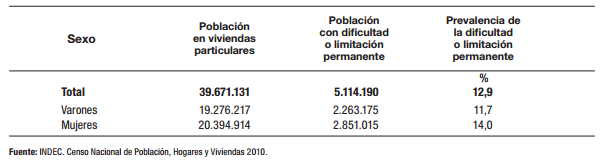
\includegraphics{Figures/porcentaje_discapacitad_por_sexo}
\decoRule
\caption[]{Población con dificultad o limitación permanente y
prevalencia de la dificultad o limitación permanente, por sexo. Año 2010}
\label{fig:porcentaje_discapacitad_por_sexo}
\end{figure}

Concentrándonos en la parte de la población que presenta alguna dificultad visual, el censo obtuvo como resultado que la distribución porcentual
con tal dificultad representa el 59,9 de la población con dificultades, mientras que el resto de las dificultades (Motora superior, Motora inferior, Cognitiva y Auditiva)
se reparten en proporciones casi iguales.

\begin{figure}[H]
\centering
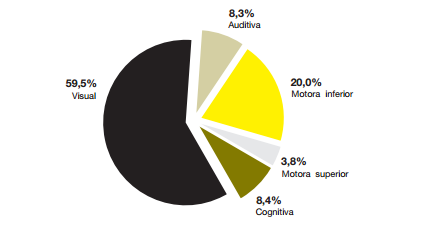
\includegraphics{Figures/poblacion_discapacidad_porcentaje}
\decoRule
\caption[]{Distribución porcentual de la población con una sola dificultad o limitación permanente por tipo de dificultad. Total del país. Año 2010}
\label{fig:poblacion_discapacidad_porcentaje}
\end{figure}

Por lo tanto, la cantidad de personas con discapacidades visuales fue de 3.063.399 en el año 2010. Por otra parte, el 90,2 por ciento de la población concurre
 o concurrió a un establecimiento educativo común, no de educación especial, al que solo fue o va el 9,8 de los encuestados. 
 El 26,1 por ciento de los encuestados usa computadora, y es la población de entre 6 y 29 años la que más lo usa.
 
La inclusión a la educación es realmente un importante tópico para poder incrementar estos números, aportar a la inclusión ayudará a la población 
a insertarse en los distintos niveles educativos.

%---------------------------------------------------------------------------------------

\section{Alcance de la tesis}

Se desea construir una prueba de concepto (PoC) que intente resolver el problema planteado. 
Esta PoC busca entender diferentes entradas:
\begin{itemize}
\item una expresión matemática escrita en \textbf{\LaTeX{}}
\item una expresión matemática escrita en \textbf{MathML}
\item \textbf{archivo} que contenga expresiones matemáticas escritas en \LaTeX{}.
\end{itemize}
Dado cualquiera de estas entradas, la PoC hará traducción al lenguaje natural en español de las expresiones matemáticas y será devuelto en texto.
Además, la PoC asumirá la existencia de un convertor de LaTeX a MathML (adelante en el documento se explicará la necesidad de éste componente), y no generará TTS. \
Ésta PoC busca que funcione modularmente entre las distintas entradas y el sistema TTS preferido por el usuario.

%---------------------------------------------------------------------------------------

\section{Estructura de la tesis}

El siguiente documento de tesis se divide en cinco secciones principales. En la sección 1 (y actual) se mencionará una introducción al documento de tesis, le brindará al lector una idea introductoria del problema que la tesis busca resolver, a su vez, busca dar un contexto social al problema y la importancia de su solución. A su vez, esta sección busca definir qué alcance tendrá el documento y su proyecto asociado.

En la sección 2 \textit{- Análisis de tipos de entrada -} se muestra un análisis de cómo iniciar a encarar el problema que se quiere resolver. Mostrando qué tipos de entradas son las que manipula los sujetos involucrados. También, esta sección, busca desarrollar con el lector los términos y definiciones que serán utilizados a lo largo del documento, conocer en detalle qué ofrece y qué no ofrece cada entrada. Y finalmente, mostrar los argumentos que llevan a la desición de cómo iniciar el proceso de desarrollo de la solución.

En la sección 3, - \textit{Arquitectura de la solución} -, busca mostrarle al lector cuáles partes están involucradas y que conjunamente forman a la solución final. Esta seccion define los distintos alcances, objetivos, acciones, comportamiento de cada componente. A su vez, quiere desplegar la manera en la que estos componentes se comunican.

En la sección 4, llamada \textit{Construcción y evaluación de la gramática}, despliega al lector los mecanismos empleados para la construcción de éste verbalizador que busca mejorar la accesibilidad de la matemática y a su vez, muestra al lector 3 maneras de evaluar el verbalizador. El objetivo de ésta sección es poder mostrar cómo el verbalizador puede mejorar para que se asemeje cada vez mas a cómo nosotros mismos dictaríamos una expresión matemática a una persona que no puede verla.

Finalmente si bien los anexos no son una sección en particular aquí está presente toda la evidencia de la que el resto del documento cita y se basa. Intenta que el lector tenga más contexto si desea averiguar un poco más acerca de lo que está leyendo.

\begin{comment}
\subsection{A (not so short) Introduction to \LaTeX{}}
If you are new to \LaTeX{}, there is a very good eBook -- freely available online as a PDF file -- called, \enquote{The Not So Short Introduction to \LaTeX{}}. The book's title is typically shortened to just \emph{lshort}. You can download the latest version (as it is occasionally updated) from here:
\url{http://www.ctan.org/tex-archive/info/lshort/english/lshort.pdf}

It is also available in several other languages. Find yours from the list on this page: \url{http://www.ctan.org/tex-archive/info/lshort/}

It is recommended to take a little time out to learn how to use \LaTeX{} by creating several, small `test' documents, or having a close look at several templates on:\\
\url{http://www.LaTeXTemplates.com}\\
Making the effort now means you're not stuck learning the system when what you \emph{really} need to be doing is writing your thesis.

\subsection{A Short Math Guide for \LaTeX{}}

If you are writing a technical or mathematical thesis, then you may want to read the document by the AMS (American Mathematical Society) called, \enquote{A Short Math Guide for \LaTeX{}}. It can be found online here:
\url{http://www.ams.org/tex/amslatex.html}
under the \enquote{Additional Documentation} section towards the bottom of the page.

\subsection{Common \LaTeX{} Math Symbols}
There are a multitude of mathematical symbols available for \LaTeX{} and it would take a great effort to learn the commands for them all. The most common ones you are likely to use are shown on this page:
\url{http://www.sunilpatel.co.uk/latex-type/latex-math-symbols/}

You can use this page as a reference or crib sheet, the symbols are rendered as large, high quality images so you can quickly find the \LaTeX{} command for the symbol you need.

\subsection{\LaTeX{} on a Mac}

The \LaTeX{} distribution is available for many systems including Windows, Linux and Mac OS X. The package for OS X is called MacTeX and it contains all the applications you need -- bundled together and pre-customized -- for a fully working \LaTeX{} environment and work flow.

MacTeX includes a custom dedicated \LaTeX{} editor called TeXShop for writing your `\file{.tex}' files and BibDesk: a program to manage your references and create your bibliography section just as easily as managing songs and creating playlists in iTunes.

%----------------------------------------------------------------------------------------

\section{Getting Started with this Template}

If you are familiar with \LaTeX{}, then you should explore the directory structure of the template and then proceed to place your own information into the \emph{THESIS INFORMATION} block of the \file{main.tex} file. You can then modify the rest of this file to your unique specifications based on your degree/university. Section \ref{FillingFile} on page \pageref{FillingFile} will help you do this. Make sure you also read section \ref{ThesisConventions} about thesis conventions to get the most out of this template.

If you are new to \LaTeX{} it is recommended that you carry on reading through the rest of the information in this document.

Before you begin using this template you should ensure that its style complies with the thesis style guidelines imposed by your institution. In most cases this template style and layout will be suitable. If it is not, it may only require a small change to bring the template in line with your institution's recommendations. These modifications will need to be done on the \file{MastersDoctoralThesis.cls} file.

\subsection{About this Template}

This \LaTeX{} Thesis Template is originally based and created around a \LaTeX{} style file created by Steve R.\ Gunn from the University of Southampton (UK), department of Electronics and Computer Science. You can find his original thesis style file at his site, here:
\url{http://www.ecs.soton.ac.uk/~srg/softwaretools/document/templates/}

Steve's \file{ecsthesis.cls} was then taken by Sunil Patel who modified it by creating a skeleton framework and folder structure to place the thesis files in. The resulting template can be found on Sunil's site here:
\url{http://www.sunilpatel.co.uk/thesis-template}

Sunil's template was made available through \url{http://www.LaTeXTemplates.com} where it was modified many times based on user requests and questions. Version 2.0 and onwards of this template represents a major modification to Sunil's template and is, in fact, hardly recognisable. The work to make version 2.0 possible was carried out by \href{mailto:vel@latextemplates.com}{Vel} and Johannes Böttcher.

%----------------------------------------------------------------------------------------

\section{What this Template Includes}

\subsection{Folders}

This template comes as a single zip file that expands out to several files and folders. The folder names are mostly self-explanatory:

\keyword{Appendices} -- this is the folder where you put the appendices. Each appendix should go into its own separate \file{.tex} file. An example and template are included in the directory.

\keyword{Chapters} -- this is the folder where you put the thesis chapters. A thesis usually has about six chapters, though there is no hard rule on this. Each chapter should go in its own separate \file{.tex} file and they can be split as:
\begin{itemize}
\item Chapter 1: Introduction to the thesis topic
\item Chapter 2: Background information and theory
\item Chapter 3: (Laboratory) experimental setup
\item Chapter 4: Details of experiment 1
\item Chapter 5: Details of experiment 2
\item Chapter 6: Discussion of the experimental results
\item Chapter 7: Conclusion and future directions
\end{itemize}
This chapter layout is specialised for the experimental sciences.

\keyword{Figures} -- this folder contains all figures for the thesis. These are the final images that will go into the thesis document.

\subsection{Files}

Included are also several files, most of them are plain text and you can see their contents in a text editor. After initial compilation, you will see that more auxiliary files are created by \LaTeX{} or BibTeX and which you don't need to delete or worry about:

\keyword{example.bib} -- this is an important file that contains all the bibliographic information and references that you will be citing in the thesis for use with BibTeX. You can write it manually, but there are reference manager programs available that will create and manage it for you. Bibliographies in \LaTeX{} are a large subject and you may need to read about BibTeX before starting with this. Many modern reference managers will allow you to export your references in BibTeX format which greatly eases the amount of work you have to do.

\keyword{MastersDoctoralThesis.cls} -- this is an important file. It is the class file that tells \LaTeX{} how to format the thesis.

\keyword{main.pdf} -- this is your beautifully typeset thesis (in the PDF file format) created by \LaTeX{}. It is supplied in the PDF with the template and after you compile the template you should get an identical version.

\keyword{main.tex} -- this is an important file. This is the file that you tell \LaTeX{} to compile to produce your thesis as a PDF file. It contains the framework and constructs that tell \LaTeX{} how to layout the thesis. It is heavily commented so you can read exactly what each line of code does and why it is there. After you put your own information into the \emph{THESIS INFORMATION} block -- you have now started your thesis!

Files that are \emph{not} included, but are created by \LaTeX{} as auxiliary files include:

\keyword{main.aux} -- this is an auxiliary file generated by \LaTeX{}, if it is deleted \LaTeX{} simply regenerates it when you run the main \file{.tex} file.

\keyword{main.bbl} -- this is an auxiliary file generated by BibTeX, if it is deleted, BibTeX simply regenerates it when you run the \file{main.aux} file. Whereas the \file{.bib} file contains all the references you have, this \file{.bbl} file contains the references you have actually cited in the thesis and is used to build the bibliography section of the thesis.

\keyword{main.blg} -- this is an auxiliary file generated by BibTeX, if it is deleted BibTeX simply regenerates it when you run the main \file{.aux} file.

\keyword{main.lof} -- this is an auxiliary file generated by \LaTeX{}, if it is deleted \LaTeX{} simply regenerates it when you run the main \file{.tex} file. It tells \LaTeX{} how to build the \emph{List of Figures} section.

\keyword{main.log} -- this is an auxiliary file generated by \LaTeX{}, if it is deleted \LaTeX{} simply regenerates it when you run the main \file{.tex} file. It contains messages from \LaTeX{}, if you receive errors and warnings from \LaTeX{}, they will be in this \file{.log} file.

\keyword{main.lot} -- this is an auxiliary file generated by \LaTeX{}, if it is deleted \LaTeX{} simply regenerates it when you run the main \file{.tex} file. It tells \LaTeX{} how to build the \emph{List of Tables} section.

\keyword{main.out} -- this is an auxiliary file generated by \LaTeX{}, if it is deleted \LaTeX{} simply regenerates it when you run the main \file{.tex} file.

So from this long list, only the files with the \file{.bib}, \file{.cls} and \file{.tex} extensions are the most important ones. The other auxiliary files can be ignored or deleted as \LaTeX{} and BibTeX will regenerate them.

%----------------------------------------------------------------------------------------

\section{Filling in Your Information in the \file{main.tex} File}\label{FillingFile}

You will need to personalise the thesis template and make it your own by filling in your own information. This is done by editing the \file{main.tex} file in a text editor or your favourite LaTeX environment.

Open the file and scroll down to the second large block titled \emph{THESIS INFORMATION} where you can see the entries for \emph{University Name}, \emph{Department Name}, etc \ldots

Fill out the information about yourself, your group and institution. You can also insert web links, if you do, make sure you use the full URL, including the \code{http://} for this. If you don't want these to be linked, simply remove the \verb|\href{url}{name}| and only leave the name.

When you have done this, save the file and recompile \code{main.tex}. All the information you filled in should now be in the PDF, complete with web links. You can now begin your thesis proper!

%----------------------------------------------------------------------------------------

\section{The \code{main.tex} File Explained}

The \file{main.tex} file contains the structure of the thesis. There are plenty of written comments that explain what pages, sections and formatting the \LaTeX{} code is creating. Each major document element is divided into commented blocks with titles in all capitals to make it obvious what the following bit of code is doing. Initially there seems to be a lot of \LaTeX{} code, but this is all formatting, and it has all been taken care of so you don't have to do it.

Begin by checking that your information on the title page is correct. For the thesis declaration, your institution may insist on something different than the text given. If this is the case, just replace what you see with what is required in the \emph{DECLARATION PAGE} block.

Then comes a page which contains a funny quote. You can put your own, or quote your favourite scientist, author, person, and so on. Make sure to put the name of the person who you took the quote from.

Following this is the abstract page which summarises your work in a condensed way and can almost be used as a standalone document to describe what you have done. The text you write will cause the heading to move up so don't worry about running out of space.

Next come the acknowledgements. On this page, write about all the people who you wish to thank (not forgetting parents, partners and your advisor/supervisor).

The contents pages, list of figures and tables are all taken care of for you and do not need to be manually created or edited. The next set of pages are more likely to be optional and can be deleted since they are for a more technical thesis: insert a list of abbreviations you have used in the thesis, then a list of the physical constants and numbers you refer to and finally, a list of mathematical symbols used in any formulae. Making the effort to fill these tables means the reader has a one-stop place to refer to instead of searching the internet and references to try and find out what you meant by certain abbreviations or symbols.

The list of symbols is split into the Roman and Greek alphabets. Whereas the abbreviations and symbols ought to be listed in alphabetical order (and this is \emph{not} done automatically for you) the list of physical constants should be grouped into similar themes.

The next page contains a one line dedication. Who will you dedicate your thesis to?

Finally, there is the block where the chapters are included. Uncomment the lines (delete the \code{\%} character) as you write the chapters. Each chapter should be written in its own file and put into the \emph{Chapters} folder and named \file{Chapter1}, \file{Chapter2}, etc\ldots Similarly for the appendices, uncomment the lines as you need them. Each appendix should go into its own file and placed in the \emph{Appendices} folder.

After the preamble, chapters and appendices finally comes the bibliography. The bibliography style (called \option{authoryear}) is used for the bibliography and is a fully featured style that will even include links to where the referenced paper can be found online. Do not underestimate how grateful your reader will be to find that a reference to a paper is just a click away. Of course, this relies on you putting the URL information into the BibTeX file in the first place.

%----------------------------------------------------------------------------------------

\section{Thesis Features and Conventions}\label{ThesisConventions}

To get the best out of this template, there are a few conventions that you may want to follow.

One of the most important (and most difficult) things to keep track of in such a long document as a thesis is consistency. Using certain conventions and ways of doing things (such as using a Todo list) makes the job easier. Of course, all of these are optional and you can adopt your own method.

\subsection{Printing Format}

This thesis template is designed for double sided printing (i.e. content on the front and back of pages) as most theses are printed and bound this way. Switching to one sided printing is as simple as uncommenting the \option{oneside} option of the \code{documentclass} command at the top of the \file{main.tex} file. You may then wish to adjust the margins to suit specifications from your institution.

The headers for the pages contain the page number on the outer side (so it is easy to flick through to the page you want) and the chapter name on the inner side.

The text is set to 11 point by default with single line spacing, again, you can tune the text size and spacing should you want or need to using the options at the very start of \file{main.tex}. The spacing can be changed similarly by replacing the \option{singlespacing} with \option{onehalfspacing} or \option{doublespacing}.

\subsection{Using US Letter Paper}

The paper size used in the template is A4, which is the standard size in Europe. If you are using this thesis template elsewhere and particularly in the United States, then you may have to change the A4 paper size to the US Letter size. This can be done in the margins settings section in \file{main.tex}.

Due to the differences in the paper size, the resulting margins may be different to what you like or require (as it is common for institutions to dictate certain margin sizes). If this is the case, then the margin sizes can be tweaked by modifying the values in the same block as where you set the paper size. Now your document should be set up for US Letter paper size with suitable margins.

\subsection{References}

The \code{biblatex} package is used to format the bibliography and inserts references such as this one \parencite{Reference1}. The options used in the \file{main.tex} file mean that the in-text citations of references are formatted with the author(s) listed with the date of the publication. Multiple references are separated by semicolons (e.g. \parencite{Reference2, Reference1}) and references with more than three authors only show the first author with \emph{et al.} indicating there are more authors (e.g. \parencite{Reference3}). This is done automatically for you. To see how you use references, have a look at the \file{Chapter1.tex} source file. Many reference managers allow you to simply drag the reference into the document as you type.

Scientific references should come \emph{before} the punctuation mark if there is one (such as a comma or period). The same goes for footnotes\footnote{Such as this footnote, here down at the bottom of the page.}. You can change this but the most important thing is to keep the convention consistent throughout the thesis. Footnotes themselves should be full, descriptive sentences (beginning with a capital letter and ending with a full stop). The APA6 states: \enquote{Footnote numbers should be superscripted, [...], following any punctuation mark except a dash.} The Chicago manual of style states: \enquote{A note number should be placed at the end of a sentence or clause. The number follows any punctuation mark except the dash, which it precedes. It follows a closing parenthesis.}

The bibliography is typeset with references listed in alphabetical order by the first author's last name. This is similar to the APA referencing style. To see how \LaTeX{} typesets the bibliography, have a look at the very end of this document (or just click on the reference number links in in-text citations).

\subsubsection{A Note on bibtex}

The bibtex backend used in the template by default does not correctly handle unicode character encoding (i.e. "international" characters). You may see a warning about this in the compilation log and, if your references contain unicode characters, they may not show up correctly or at all. The solution to this is to use the biber backend instead of the outdated bibtex backend. This is done by finding this in \file{main.tex}: \option{backend=bibtex} and changing it to \option{backend=biber}. You will then need to delete all auxiliary BibTeX files and navigate to the template directory in your terminal (command prompt). Once there, simply type \code{biber main} and biber will compile your bibliography. You can then compile \file{main.tex} as normal and your bibliography will be updated. An alternative is to set up your LaTeX editor to compile with biber instead of bibtex, see \href{http://tex.stackexchange.com/questions/154751/biblatex-with-biber-configuring-my-editor-to-avoid-undefined-citations/}{here} for how to do this for various editors.

\subsection{Tables}

Tables are an important way of displaying your results, below is an example table which was generated with this code:

{\small
\begin{verbatim}
\begin{table}
\caption{The effects of treatments X and Y on the four groups studied.}
\label{tab:treatments}
\centering
\begin{tabular}{l l l}
\toprule
\tabhead{Groups} & \tabhead{Treatment X} & \tabhead{Treatment Y} \\
\midrule
1 & 0.2 & 0.8\\
2 & 0.17 & 0.7\\
3 & 0.24 & 0.75\\
4 & 0.68 & 0.3\\
\bottomrule\\
\end{tabular}
\end{table}
\end{verbatim}
}

\begin{table}
\caption{The effects of treatments X and Y on the four groups studied.}
\label{tab:treatments}
\centering
\begin{tabular}{l l l}
\toprule
\tabhead{Groups} & \tabhead{Treatment X} & \tabhead{Treatment Y} \\
\midrule
1 & 0.2 & 0.8\\
2 & 0.17 & 0.7\\
3 & 0.24 & 0.75\\
4 & 0.68 & 0.3\\
\bottomrule\\
\end{tabular}
\end{table}

You can reference tables with \verb|\ref{<label>}| where the label is defined within the table environment. See \file{Chapter1.tex} for an example of the label and citation (e.g. Table~\ref{tab:treatments}).

\subsection{Figures}

There will hopefully be many figures in your thesis (that should be placed in the \emph{Figures} folder). The way to insert figures into your thesis is to use a code template like this:
\begin{verbatim}
\begin{figure}
\centering
\includegraphics{Figures/Electron}
\decoRule
\caption[An Electron]{An electron (artist's impression).}
\label{fig:Electron}
\end{figure}
\end{verbatim}
Also look in the source file. Putting this code into the source file produces the picture of the electron that you can see in the figure below.

\begin{figure}[H]
\centering
\includegraphics{Figures/Electron}
\decoRule
\caption[An Electron]{An electron (artist's impression).}
\label{fig:Electron}
\end{figure}

Sometimes figures don't always appear where you write them in the source. The placement depends on how much space there is on the page for the figure. Sometimes there is not enough room to fit a figure directly where it should go (in relation to the text) and so \LaTeX{} puts it at the top of the next page. Positioning figures is the job of \LaTeX{} and so you should only worry about making them look good!

Figures usually should have captions just in case you need to refer to them (such as in Figure~\ref{fig:Electron}). The \verb|\caption| command contains two parts, the first part, inside the square brackets is the title that will appear in the \emph{List of Figures}, and so should be short. The second part in the curly brackets should contain the longer and more descriptive caption text.

The \verb|\decoRule| command is optional and simply puts an aesthetic horizontal line below the image. If you do this for one image, do it for all of them.

\LaTeX{} is capable of using images in pdf, jpg and png format.

\subsection{Typesetting mathematics}

If your thesis is going to contain heavy mathematical content, be sure that \LaTeX{} will make it look beautiful, even though it won't be able to solve the equations for you.

The \enquote{Not So Short Introduction to \LaTeX} (available on \href{http://www.ctan.org/tex-archive/info/lshort/english/lshort.pdf}{CTAN}) should tell you everything you need to know for most cases of typesetting mathematics. If you need more information, a much more thorough mathematical guide is available from the AMS called, \enquote{A Short Math Guide to \LaTeX} and can be downloaded from:
\url{ftp://ftp.ams.org/pub/tex/doc/amsmath/short-math-guide.pdf}

There are many different \LaTeX{} symbols to remember, luckily you can find the most common symbols in \href{http://ctan.org/pkg/comprehensive}{The Comprehensive \LaTeX~Symbol List}.

You can write an equation, which is automatically given an equation number by \LaTeX{} like this:
\begin{verbatim}
\begin{equation}
E = mc^{2}
\label{eqn:Einstein}
\end{equation}
\end{verbatim}

This will produce Einstein's famous energy-matter equivalence equation:
\begin{equation}
E = mc^{2}
\label{eqn:Einstein}
\end{equation}

All equations you write (which are not in the middle of paragraph text) are automatically given equation numbers by \LaTeX{}. If you don't want a particular equation numbered, use the unnumbered form:
\begin{verbatim}
\[ a^{2}=4 \]
\end{verbatim}

%----------------------------------------------------------------------------------------

\section{Sectioning and Subsectioning}

You should break your thesis up into nice, bite-sized sections and subsections. \LaTeX{} automatically builds a table of Contents by looking at all the \verb|\chapter{}|, \verb|\section{}|  and \verb|\subsection{}| commands you write in the source.

The Table of Contents should only list the sections to three (3) levels. A \verb|chapter{}| is level zero (0). A \verb|\section{}| is level one (1) and so a \verb|\subsection{}| is level two (2). In your thesis it is likely that you will even use a \verb|subsubsection{}|, which is level three (3). The depth to which the Table of Contents is formatted is set within \file{MastersDoctoralThesis.cls}. If you need this changed, you can do it in \file{main.tex}.

%----------------------------------------------------------------------------------------

\section{In Closing}

You have reached the end of this mini-guide. You can now rename or overwrite this pdf file and begin writing your own \file{Chapter1.tex} and the rest of your thesis. The easy work of setting up the structure and framework has been taken care of for you. It's now your job to fill it out!

Good luck and have lots of fun!

\begin{flushright}
Guide written by ---\\
Sunil Patel: \href{http://www.sunilpatel.co.uk}{www.sunilpatel.co.uk}\\
Vel: \href{http://www.LaTeXTemplates.com}{LaTeXTemplates.com}
\end{flushright}

\end{comment}

% Chapter Template

\chapter{Análisis de tipos de entrada}

\label{Chapter2} % Change X to a consecutive number; for referencing this chapter elsewhere, use \ref{ChapterX}

%----------------------------------------------------------------------------------------

\section{MathML}


\subsection{¿Qué es MathML?}

MathML (Mathematical Markup Language) \cite{2} es un dialecto XML para describir notaciones matemáticas que busca capturar tanto la estructura
como el contenido. Su objetivo es integrar las fórmulas matemáticas en las páginas de Internet y otros documentos.
Forma parte de HTML5 y de un estándar ISO ISO/IEC DIS 40314 desde el año 2015.

Una de las ventajas de MathML es que es un estándar de representación de fórmulas matemáticas para la World Wide Web (W3) y los principales y más usados
navegadores de Internet tienen integrado de manera nativa el soporte para éste tipo de contenido haciéndolo una aplicación accesible.

MathML consiste de un número de tags XML que pueden ser usados
para el marcado de una ecuación en términos de su representación y su semántica. Ésto último es sumamente importante
ya que MathML busca capturar el significado detrás de la ecuación además de concentrarse en cómo ésta será formateada y mostrada en pantalla.

MathML busca facilitar el uso y el re uso de contenido científico en la Web. La versatilidad de éste lenguaje de marcado nos permite aprovechar
su notación para displays visuales de alta calidad y su contenido para aplicaciones más semánticas cómo software científico o sintetizadores de voz.

Como se mencionó MathML codifica tanto la estructura como el contenido de las expresiones matemáticas.
A través del marcado de presentación (Presentation MathML o PMathML) se pueden desplegar expresiones matemáticas, y mediante el marcado de contenido
(Content MathML o CMathML) se puede representar el significado de las expresiones matemáticas.

\subsection{PMathML}

El \textbf{marcado de presentación} tiene como objetivo principal describir la estructura de una fórmula matemática.
Los elementos de presentación corresponden a los \textbf{constructores} de la notación matemática tradicional, en la última versión de MathML se incluyen
37 tags que pueden ser usados para representar una fórmula matemática. Los tags más usados son \textit{<mi>, <mo>, <mrow>} para indicar una \textit{variables, operadores,
expresiones anidadas}, respectivamente.

\subsection{CMathML}

El \textbf{marcado de contenido} tiene como objetivo principal describir la semántica de una fórmula matemática.
Provee una lista mucho más amplia de tags para ser usados con respecto a PMathML, sumando un total de 129.
Entre los tags más usados tenemos <apply>, <ci>, <cn>. El primero de ellos se utiliza para hacer explícita la aplicación de un
operador a sus children's (tags hijos), dejando en claro cuál es el scope de aplicación. El segundo tag se utiliza para describir variables y el tercero
de ellos se utiliza para describir los números. CMathML contiene un tag en específico para cada operación matemática, lo que lo hace más específico que PMathML
ya que PMathML contiene un tag solo para algunas operaciones (como la suma o multiplicación).

En la siguiente figura se puede observar cómo se describe en PMathML y CMathML para la siguiente fórmula matemática: $x + \frac{a}{b}$

\begin{figure}[H]
\centering
  \begin{minipage}[b]{0.4\textwidth}
    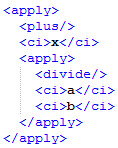
\includegraphics{Figures/ejemplo_cmathml}
    \caption[]{CMathML}
  \end{minipage}
  \begin{minipage}[b]{0.4\textwidth}
    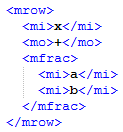
\includegraphics{Figures/ejemplo_pmathml}
    \caption[]{PMathML}
  \end{minipage}
\label{fig:ejemplo_cmathml}
\end{figure}

\subsection{¿Por qué CMathML?}
Hay ciertas expresiones matemáticas que pueden tener distintas interpretaciones, esto la hace una expresión ambigua, ya que muchas veces
depende del contexto su correcta interpretación. Supongamos la siguiente fórmula matemática:
$$f^{-1}$$
Que puede interpretarse como la función inversa de f o, también como, la variable f elevado a -1. Para ello veamos cómo es su marcado tanto en PMathML como en CMathML.
Para PMathML tenemos el siguiente XML:
\lstset{language=XML}
\begin{lstlisting}
<math xmlns="http://www.w3.org/1998/Math/MathML">
  <msup>
    <mi>f</mi>
    <mn>-1</mn>
  </msup>
</math>
\end{lstlisting}

Podemos ver que, dado que PMathML intenta solo capturar su presentación, su XML asociado sigue siendo ambiguo. Ya que la etiqueta \textit{<msup>} solo
señala que -1 es el superíndice de f. Lo que lo vuelve ambiguo tal como se escribe su expresión matemática.

En cambio para CMathML, ya que ésta intenta capturar su semántica, podemos ver que tenemos dos posibles XML asociados a esta fórmula matemática.

\lstset{language=XML}
\begin{lstlisting}
<math xmlns="http://www.w3.org/1998/Math/MathML">
  <apply>
    <inverse/>
    <ci type="function">f</ci>
  </apply>
</math>
\end{lstlisting}

y también tenemos

\lstset{language=XML}
\begin{lstlisting}
<math xmlns="http://www.w3.org/1998/Math/MathML">
  <apply>
    <power/>
    <ci type="function">f</ci>
    <cn>-1</cn>
  </apply>
</math>
\end{lstlisting}

Podemos ver que para CMathML queda claro de qué interpretación queremos asociar al XML. Ya que en el primer caso tenemos el tag \textit{<inverse>}
aplicado a la variable \textit{f} que habla de la inversa de f. Y en el segundo tenemos el tag \textit{<power>} que denota el exponente \textit{-1} aplicado a \textit{f}.

Otra ventaja que tiene CMathML sobre PMathML es que existen herramientas para hacer el pasaje de CMathML a PMathML, pero debido a la ambiguedad de PMathML no existe una herramienta que lo haga en la otra dirección.

Esta es la razón principal que CMathML es el adecuado para la PoC que acompaña este trabajo final, es el lenguaje de marcado
que más se acerca a la lectura en lenguaje natural.

\section{\LaTeX}

\subsection{¿Qué es \LaTeX ?}

Según Wikipedia, \LaTeX\ es un sistema de composición de textos, orientado a la creación de documentos escritos que
presenten una alta calidad tipográfica. Por sus características y posibilidades, es usado de forma especialmente intensa en la
generación de artículos y libros científicos que incluyen, entre otros elementos, expresiones matemáticas.

Lo cierto es que \LaTeX posee a su disposición muchos paquetes para ser importados que hacen más fácil la escritura de
expresiones matemáticas. Cualquier expresión matemática puede ser escrita usando \LaTeX.

Latex fue diseñado específicamente para ser escrito por humanos por eso éste sistema es el más usado para la generación de archivos científicos y, por lo tanto, muchas expresiones matemáticas
son escritas con \LaTeX, lo que hace que \LaTeX sea el lenguaje más usado para escribir éste tipo de expresiones.
Si bien MathML es usado por distintos softwares científicos y navegadores web, no es realmente el lenguaje más usado para escribir expresiones matemáticas desde
el lado del usuario, como lo es \LaTeX.

Esta es la razón por la que \LaTeX es considerado como un tipo de entrada válido para la PoC.

A modo ilustrativo, veamos cómo es en sintaxis \LaTeX la fórmula $x + \frac{a}{b}$:

\verb|$x + \frac{a}{b}$|

Podemos notar que, al igual que CMathML, captura la estructura y el contenido de la expresión. Sabiendo que \verb|\frac| es la manera de escribir una fracción y con \textit{+} podemos escrbir la suma, podemos leer con facilidad la expresión matemática mencionada y darle el respectivo significado. Cabe mencionar, que hay una relación entre CMathML y \LaTeX y será explicado más adelante en este documento.

\LaTeX además de ser usado ampliamente por científicos para escribir sus publicaciones y documentos, también es usado para describir
algunas expresiones matemáticas en Internet. Tal es así el caso de Wikipedia, que para cada fórmula matemática que tenga presente en algún artículo en línea posee dentro de el atributo \textit{alt} del tag \textit{<img>}
su descripción en lenguaje \LaTeX.

Por ejemplo, veamos en el artículo que explica las ecuaciones de segundo grado %(Cita: https: es.wikipedia.org wiki Ecuación_de_segundo_grado) en su segunda figura tenemos
$$x = \frac{-b \pm \sqrt {b^2-4ac}}{2a}$$

mientras que su código HTML tenemos
\\
\verb|<img|\\
\verb|  class="tex" src="expresion.png"|\\
\verb|  alt="x = \frac{-b \pm \sqrt {b^2-4ac}}{2a}"|\\
\verb|>|

\subsection{Análisis de \LaTeX y MathML}

Si bien la relación entre Latex y CMathML\cite{5} es muy sensible y fina, existe. Comencemos diferenciado éstas tecnologías desde un punto de vista de usabilidad y comprensión, así también desde tipo de entrada.

\begin{itemize}
\item \textbf{Usabilidad}: Latex es el lenguaje más usado para escribir documentos y artículos científicos, hay tutoriales y documentación con ejemplos para aprender a escribir usando este lenguaje. Latex funciona desde el lado del usuario (\textit{user-side}), mientras que MathML es la aplicación más usada para renderizar expresiones matemáticas en distintos softwares, y funciona desde el lado del servidor (\textit{server-side}). En muchos artículos se menciona que MathML es la representación que las computadoras entienden de las expresiones que conocemos.
\item \textbf{Compresión desde el usuario}: Una expresión matemática, tanto escrita con Latex o MathML, pueden ser leídas con el mismo grado de dificultad. Si la expresión es más avanzada, la lectura desde un humano puede requerir un poco más de atención. Pero a la hora de la escritura, Latex es más amigable que MathML.
\item \textbf{Tipo de entrada}: MathML saca ventaja sobre Latex de ésto ya que, como se mencionó, MathML es un dialecto XML que nos permite renderizar cualquier expresión matemática y consigo trae todas las ventajas que tiene una aplicación XML. El parser es un componente estándar, por lo tanto no es necesario crear un parser específico para cada versión de lenguaje XML. Esto posibilita el empleo de cualquiera de los analizadores disponibles. De esta manera se evitan bugs y se acelera el desarrollo de aplicaciones. Pero no funciona así con Latex, debido que Latex es un lenguaje de programación y no un estándar puede ser extendido por lo tanto no hay un parser disponible para poder particionar una expresión latex para procesar partes más atómicas.
\end{itemize}

Las conclusiones hasta el momento es que Latex es el lenguaje más elegido por los usuarios y MathML es la aplicación más elegida para desarrollar el software. Es por eso que en ésta tesis se intenta hacer un ligamento entre éstas tecnologías y aprovechar las ventajas de cada uno. 
% Chapter Template

\chapter{Arquitectura de la solución} % Main chapter title

\label{Chapter3} % Change X to a consecutive number; for referencing this chapter elsewhere, use \ref{ChapterX}

%----------------------------------------------------------------------------------------
%  SECTION 1
%----------------------------------------------------------------------------------------

\section{Entrada y salida}

Se asumen tres tipos de entradas que TexToES puede entender.

\begin{itemize}
\item{\textbf{LaTeX}}

Dadas las razones explicadas anteriormente, Latex es un tipo de entrada que TexToES puede procesar e interpretar. TexToES asume que la expresión latex está encerrada entre \verb|$| para delimitar el inicio y el fin de ésta.

\textit{Ejemplo}:
$$\verb|$\max(1, 2, 3, 4) = 4$|$$

\item{\textbf{CMathML}}

Como se mencionó, CMathML captura el contenido de la expresión es por eso que se prefiere CMathML antes que PMathML. TexToES asume que la entrada viene dada con su respectiva estructura XML definida por el estándar. Por lo tanto, deberá comenzar con la etiqueta \textbf{<math>}.

\textit{Ejemplo}:
$$\textit{\textbf{<math>}<apply><eq/><ci>a</ci><ci>b</ci></apply>\textbf{</math>}}$$

\item{\textbf{Archivo que contenga expresiones latex}}

TexToES también admite cualquier archivo con extensión \textit{*.txt} que dentro contenga expresiones latex. Se debe cumplir también aquí que las expresiones están encerradas entre \verb|$|.

\end{itemize}

Para cada tipo de entrada obtenemos un texto como tipo de salida que es la representación en lenguaje natural español de la entrada selecta. Para visualizarlo mejor, tenemos el siguiente gráfico:

\begin{figure}[H]
\centering
  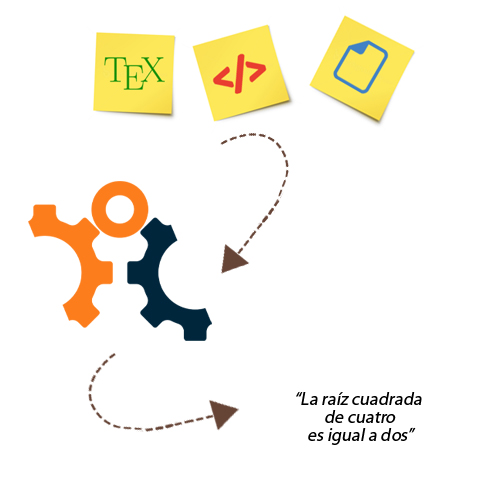
\includegraphics[width=10cm, height=10cm]{Figures/arquitectura-general-textoes}
  \caption[]{Flujo simple de TexToES}
\label{fig:arquitectura}
\end{figure}

Los engranajes representan \textbf{TexToES} y las flechas señalan la dirección del flujo. Más adelante en este documento explicaré con más detalle cómo está compuesto TexToES.

%----------------------------------------------------------------------------------------
%  SECTION 2
%----------------------------------------------------------------------------------------

\section{A favor de una solución modular}

La manera en que se encaró el desarrollo de TexToEs fue de manera tal que cada componente estuviera aislado y separado del resto.
Llevando a cabo la estrategia \textit{divide y vencerás} fue que se logró programar cada componente por separado, con una interfaz definida para que el resto de los componentes puedan comunicarse a través de ella.

Se decidió distribuir las distintas tareas identificadas en módulos para que se pueda reusar código, para poder adaptar nuevas funcionalidades y la razón más importante es poder utilizar TexToES como un único módulo a la preferencia del usuario o desarrollador.
\\[1cm]

\begin{figure}[H]
\centering
  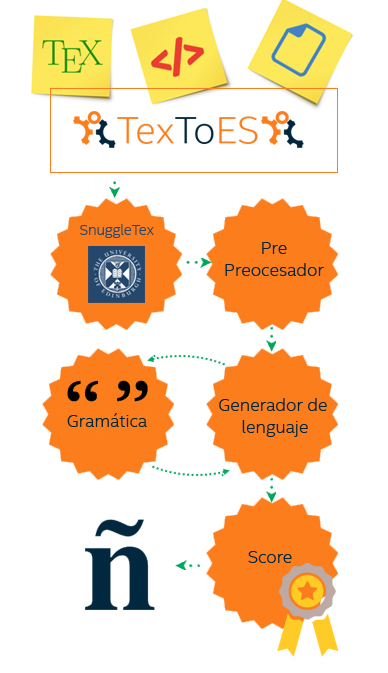
\includegraphics[width=9.22cm, height=16cm]{Figures/detalle-arqui}
  \caption[]{Gráfico de flujo de TexToES}
\label{fig:arquitectura}
\end{figure}

TexToES cuenta con cinco principales módulos los cuales son:

\begin{itemize}
\item Cliente SnuggleTeX: es el cliente que se encarga de comunicarse con el servidor SnuggleTeX, el cliente implementa una sencilla interfaz para hacer y parsear el request que convierte LaTeX a MathML. Esto entra en acción si el usuario quiere verbalizar texto LaTeX. Esta herramienta fue desarrollada por David McKain, desarrollador en School of Physics and Astronomy en la Universidad de Edimburgo.
\item Pre-procesador: Es un simple módulo que pre-procesa el MathML recibido (ya sea por el usuario o el cliente) añadiendo etiquetas y elementos que ayudan al procesamiento del XML, como resultado provee un stack que será manipulado por el verbalizador. Este módulo es desarrollo propio.
\item Verbalizador o Generador de lenguaje: Se encarga de parsear el stack que representa la fórmula matemática e ir verbalizando cada operador, constructor y constante que encuentre. Este módulo es desarrollo propio.
\item Gramática: define la gramática utilizada por el Verbalizador. Este módulo es desarrollo propio.
\item Score: Sistema que evalúa la transcripción obtenida. Indica métricas que muestran el grado de confianza de que tiene el usuario de que su verbalización obtenida esté bien. Este módulo es desarrollo propio.
\end{itemize}

La combinación de estos módulos forman a TexToES. Cabe mencionar que cada uno de ellos es exportable, i.e. el lector puede importarlos desde su ambiente de desarrollo y los puede usar por separado utilizando su interfaz.

\section{SnuggleTeX y Cliente SnuggleTeX}

SnuggleTeX\cite{3} es una librería Java gratuita y open-source para convertir fragmentos de Latex a XML (usualmente XHTML + MathML). Las funcionalidades principales que SnuggleTex provee son:

\begin{itemize}
\item SnuggleTeX convierte de código matemático simple en LaTeX a MathML, puedes obtener tanto PMathML como CMathML.
\item SnuggleTeX puede convertir el MathML resultante en imágenes (usando la librería JEuclid) y además puede convertir código MathML simple en una mezcla de XHTML y CSS.
\item SnuggleTeX puede tambien enriquecer la salida PMathML que crea, adicionalmente generando CMathML y/o Maxima.
\end{itemize}

Entre otras funcionalidades.

SnuggleTeX es un componente altamente complejo y que TexToES lo usa como un componente de caja negra, es decir, no conocemos cómo está implementado sólo utilizamos su interfaz y procesamos sus respuestas.

SnuggleTeX es quien se encarga de convertir el código LaTeX\cite{4}, que viene por entrada, a código CMathML para luego alimentar de éste al resto de los componentes para obtener la verbalización.

Dado que esta herramienta provee un mecanismo de conversión de un tipo a otro, podemos olvidarnos de la creación de un parser en específico para LaTeX que intente traducirlo a MathML, simplemente alimentos a SnuggleTeX con el código Latex que deseemos verbalizar y luego manipulamos su salida en CMathML. Actualmente, ST se encuentra hosteado en un servidor para proyectos académicos donde se puede consumir toda su funcionalidad.

Para poder alimentar y extraer la información de ST, se implementó un cliente HTTP que pueda comunicarse con el servidor que hostea a la herramienta. El cliente conoce dónde está ubicado este servidor, conoce también, las distintas URIs de cada funcionalidad y también conoce los nombres de los campos con los que ST va a consumir nuestra petición.

Comunicarse con el servidor de ST es básicamente realizar un pedido POST al servidor indicando en el campo \textit{input} el string LaTeX a convertir. Luego el cliente se encarga de parsear su respuesta para obtener el XML asociado, y en caso de que no esté presente devuelve un objeto \textbf{nulo}.

¿Cuáles son los casos en que puede no estar presente el XML asociado?

Para responder esta pregunta, nos concentramos en las limitaciones de SnuggleTeX. \\
ST tiene un rango limitado de operadores que puede soportar, si el LaTeX que le demos de entrada posee un operador o símbolo que no esté en la siguiente lista no obtendremos un resultados que podamos verbalizar.

La lista es la siguiente:

\begin{figure}[H]
\centering
  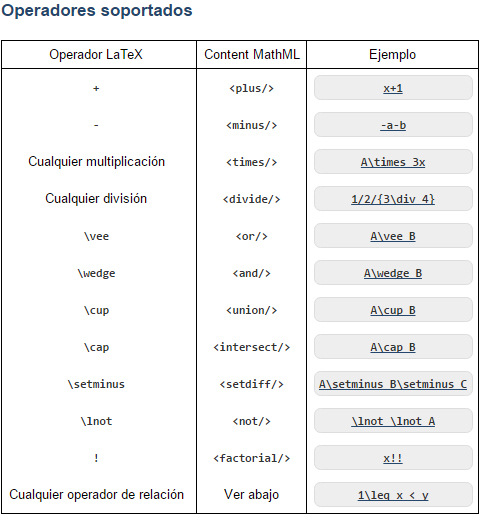
\includegraphics[width=11cm, height=11.84cm]{Figures/opsoportados}
  \caption[]{Operadores soportados por SnuggleTeX}
\label{fig:opsoportados}
\end{figure}

Para los operadores lógicos tenemos:

\begin{figure}[H]
\centering
  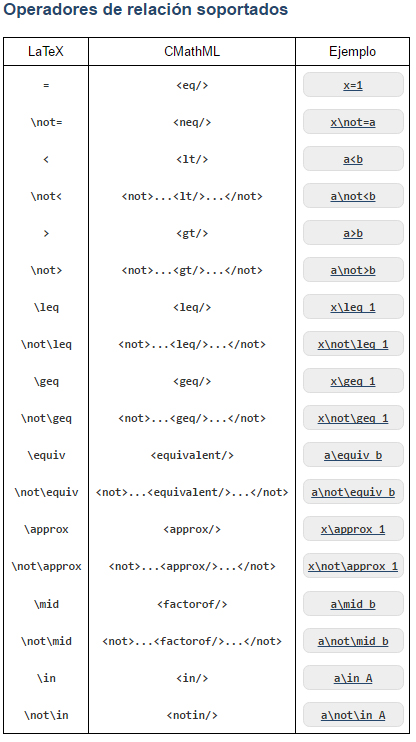
\includegraphics[width=10cm, height=17.84cm]{Figures/reloperatorsoportados}
  \caption[]{Operadores lógicos soportados por SnuggleTeX}
\label{fig:opsoportados}
\end{figure}

También ST puede parsear y dar significado en MathML para funciones pre-definidas.

\begin{tcolorbox}
\verb|\sin \cos \tan \sec \cot \sinh \cosh \lcm \ln \log|\\
\verb|\tanh \sech \csch \coth \arcsin \arccos \max \Re| \\
\verb|\arctan \arcsec \arccsc \arccot \arcsinh \min \det|\\
\verb|\arccosh \arctanh \arcsech \arccsch \gcd \Im \exp \arccoth|
\end{tcolorbox}

Quizás, en algún trabajo futuro, se pueda completar la implementación de SnuggleTeX para aquellos operadores que no estén listados aquí y así agrandar la esfera de acceso de esta herramienta.

Finalmente, TexToES utiliza ST cuando se alimente con un string que represente LaTeX. Para los casos en donde directamente dispongamos de una entrada en XML CMathML, ST no estará involucrado en este escenario.
Luego con el XML CMathML, ya sea provisto por el usuario u obtenido con el cliente de SnuggleTeX, entra en acción el siguiente módulo en el flujo.

\section{Pre-procesador}

El Pre-Procesador (o pre-processor) es el módulo más simple en TexToES pero no menos complejo. Recibe como entrada una cadena de caracteres (string) que represente un XML del tipo CMathML:\\[0.01cm]

\framebox[1.1\width]{\textit{Ejemplo:} <math><apply><eq/><ci>a</ci><ci>b</ci></apply></math>}\\[0.01cm]

Para devolver una pila (stack) con la estructura del árbol XML en una lista utilizando el método de búsqueda depth-first (DF).\\

Este último método mencionado es un algoritmo muy conocido en el área de Computación que permite recorrer todos los nodos de un árbol de manera ordenada, pero no uniforme. Su funcionamiento consiste en ir expandiendo todos y cada uno de los nodos que va localizando en un camino concreto. Cuando ya no quedan más nodos que visitar en dicho camino, regresa haciendo backtracking, de modo que repite el mismo proceso con cada uno de los hermanos del nodo ya procesado.\\

Se ha utilizado la librería estándar de Python para parsear XML (\textit{xml.etree}).\\

A medida que se recorre el árbol utilizando DF, los elementos del mismo se van apilando utilizando las siguiente reglas de aplicación:

\begin{itemize}
\item \textit{El primer nodo, identificado como "\textbf{math}", se descarta.
\item Por cada nodo etiquetado como "\textbf{apply}" se apila en el stack el string "\textbf{apply}", que es quien indica el inicio de la aplicación de un operador.
\item Por cada nodo etiquetado como "\textbf{end}", se apila en el stack el string "\textbf{end-apply}" similar al anterior, solo que con ésto podemos indicar el fin de la aplicación de la operación.
\item Cada vez que se encuentro un nodo "\textbf{ci}" o "\textbf{cn}" se apila directamente el contenido de su nodo hijo. (Recordemos que ci y cn representan números y variables respectivamente).
\item Cualquier otro caso se apila el nodo sin ninguna alteración.}
\end{itemize}

Cómo habrán notado, la etiqueta "\textbf{end}" no está presente en el string de entrada. Esto es así porque el pre-processor añade esta etiqueta para poder identificar cuando finaliza la aplicación de una operación.
Esta etiqueta custom es una etiqueta dummy su única función es identificar el final de la etiqueta "apply".

Para ello hay un algoritmo simple implementado en este módulo, podemos describir su funcionamiento en la siguiente oración:

\begin{itemize}
\item \textit{Por cada \textbf{</apply>} presente en el texto, añadiré a su izquierda lo siguiente \textbf{<end></end>}. De manera que finalmente quedará reemplazado por <end></end></apply>.}
\end{itemize}

Al finalizar, se entrega una lista (llamada stack) con el contenido del árbol recorrido en DF.\\[0.01cm]

La salida del pre-processor para el ejemplo presentado es la siguiente:\\[0.01cm]

\framebox[1.1\width]{\textit{Salida:} ['apply', 'eq', 'A', 'B', 'end-apply']}\\[0.01cm]


\section{Generador de Lenguaje}

Este módulo se encarga de verbalizar el stack que recibe desde el pre-processor. Si bien parece simple leyendo esa descripción pero es el módulo más complejo. El módulo provee una manera de generar texto basado en templates (llamado en procesamiento de lenguaje natural como template-based generators\cite{7}).

Procederé a explicar el funcionamiento de este módulo mediante un ejemplo práctico. Partamos de la siguiente expresión matemática:

$$3x - 2 = 0$$

El cual se puede representar con el siguiente CMathML:

\lstset{language=XML}
\begin{lstlisting}
<math>
   <apply>
       <eq/>
       <apply>
           <minus/>
           <apply>
               <times/>
               <cn>3</cn>
               <ci>x</ci>
           </apply>
           <cn>2</cn>
       </apply>
       <cn>0</cn>
   </apply>
</math>
\end{lstlisting}

Y el stack que obtenemos gracias al pre-processor (y entrada de este módulo) es el siguiente:\\
\framebox[\width]{ ['apply', 'eq', 'apply', 'minus', 'apply', 'times', '3',
'X', 'end-apply', '2', 'end-apply', '0', 'end-apply'] }

En rangos generales el mecanismo empleado por este módulo se puede describir con las siguientes reglas:

\begin{enumerate}
\item ¿'apply' está presente en stack?
\begin{enumerate}
  \item si no, terminar.
  \item caso contrario:
  \begin{enumerate}
     \item i es la posición de 'apply' más a la derecha en stack.
     \item j es la posición de 'end-apply' próximo a la derecha de i
     \item creo un stack temporal llamado stack\_temp que contiene el sub array desde i hasta j
     \item obtengo la operación
     \begin{enumerate}
        \item consulto en la gramática por la traducción de la operación
     \end{enumerate}
     \item obtengo su traducción desde la gramática
     \item obtengo la aridad, basándome en la cantidad de operandos en stack\_temp
     \item obtengo la verbalización de stack\_temp
     \item elimino de stack los elementos desde i hasta j y coloco su verbalización
  \end{enumerate}
  \item vuelvo al primer paso
\end{enumerate}
\end{enumerate}

Para el caso planteado podemos ver que 'apply' está presente 3 veces en el stack, por lo que el algoritmo descrito anteriormente se aplicará 3 veces.\\

{\Large \textbf{Primera iteración:}}\\
El elemento 'apply' más a la derecha presente en stack en esta iteración es el que está en la posición 4. Su end-apply próximo está en la posición 8. Por lo tanto el sub stack llamado stack\_temp es el siguiente
$$['apply', 'times', '3', 'X', 'end-apply']$$

Los datos que sé es que la operación en este stack atómico es \textbf{'times'}, su aridad es \textbf{2} y la gramática (que detallaré más adelante) nos expone que su traducción es \textbf{\$VAR\$ multiplicado por \$VAR\$} donde \$VAR\$ es un símbolo de la gramática que me puede exponer 1 o más transformaciones consecuentes. En este caso, dado que la aridad es 2, cada \$VAR\$ será reemplazado por los operados (3 y X).

La verbalización consiste simplemente en parsear la traducción desde la gramática y saber colocar desatendidamente los operados en los respectivos \$VAR\$.

Si verbalización finalmente es
$$3 multiplicado por X$$

En el stack original debemos reemplazar todos los elementos stack\_temp presentes en stack por la verbalización obtenida en esta iteración. Finalmente el siguiente es nuestro stack resultante de la primer iteración
$$['apply', 'eq', 'apply', 'minus', '(3 multiplicado por X)', '2', 'end-apply', '0', 'end-apply']$$

{\Large \textbf{Segunda iteración:\\}}
El apply siguiente se encuentra en la posición 2 y su correspondiente end-apply en la posición 6. La operación es \textbf{minus} y su aridad es también \textbf{2}. La gramática nos dice que su traducción es \textbf{\$VAR\$ menos \$VAR\$}. Finalmente su verbalización se corresponde con:
$$((3 multiplicado por X) menos 2)$$

Y el stack resultante es:
$$['apply', 'eq', '((3 multiplicado por X) menos 2)', '0', 'end-apply']$$

{\Large \textbf{Tercera iteración:\\}}
De manera análoga, obtenemos que el resultado final es
$$(((3 multiplicado por X) menos 2) es igual a 0)$$


\subsection{Gramática}

Como se ha mencionado anteriormente, este sistema que busca verbalizar, o traducir, el latex al español tiene su sistema
de generación de lenguaje natural implementado con plantillas, o lo que comúnmente se conoce como template-based generation systems.
TexToES posee una gramática donde mapea las operaciones soportadas (descritas por el operador, o función, en la etiqueta CMathML) con su representación en lenguaje natural. Es simplemente un archivo de configuración donde por cada clave (key) tenemos los operadores y en los valores (value) tenemos su representación en español.\\

La decisión por la que se llevó a cabo la implementación del template es porque se consideró que cada elemento de la etiqueta CMathML tiene una correspondencia uno a uno al español.\\

Por ejemplo, si estamos hablando de \textbf{<plus>} sabemos que estamos hablando de una suma aplicada a dos o más operados. Por lo tanto, en nuestra gramática encontraremos la siguiente línea.\\

\framebox[1.1\width]{ plus = \$VAR\$ más \$VAR\$ }\\

Dónde \$VAR\$ corresponde con símbolos terminales o con otra key dentro de la gramática. Gracias a ésto último podemos describir una suma anidada de números, o simplemente la suma de dos números.\\
Sea $\operatorname{\mathbb{T}}$ todos los elementos que denotan una variable. Por ejemplo, $x,y,f,g \in \operatorname{\mathbb{T}}$.\\
Sea $\operatorname{\mathbb{OP}}$ todos los operadores soportados por TexToES. Por ejemplo, $\textit{suma} \in \operatorname{\mathbb{OP}}$\\

Entonces, VAR en la gramática puede ser involucrar una producción del tipo:
\framebox[1.1\width]{ $VAR = \operatorname{\mathbb{R}}, \operatorname{\mathbb{T}}, \operatorname{\mathbb{OP}}$}\\

La gramática es fácil de extender, por lo tanto, si se quiere añadir soporte para algún operador no soportado, con simplemente describirla en la gramática será suficiente.

Las plantillas o templates son una forma de centralizar la representación del texto origen (source) al texto objetivo (target). Y saca su mayor provecho cuando la representación es uno a uno. Si hubiéramos seguido un approach basado en PMathML en lugar de CMathML, donde para cada PMathML podíamos tener distintas interpretaciones una gramática template-based no nos hubiera ayudado demasiado. Ya que generaríamos, algunas veces, resultados incorrectos o mal interpretados.

La gramática completa puede consultarse en el anexo de este documento.
% Chapter Template

\chapter{Construcción y evaluación de la gramática}

\label{Chapter4} % Change X to a consecutive number; for referencing this chapter elsewhere, use \ref{ChapterX}

%----------------------------------------------------------------------------------------
%  SECTION 1
%----------------------------------------------------------------------------------------

\section{Reglas de la gramática}

Como se mencionó en la sección anterior, se puede utilizar un generador de lenguaje natural o verbalizador basado en plantillas (template-based \textbf{natural language generation}). Es necesario en este punto construir templates que representen la manera más usual \textbf{o natural} de leer expresiones matemáticas \textbf{de manera que se construyan frases fidedignas al original y fáciles de comprender cuando se lean en voz alta por un lector de pantalla}. Para ello se contactó a distintos estudiantes de carreras matemáticas, e incluso Ingenieros en Sistemas y Lic. en Cs de computación para poder reconocer las distintas maneras de leer una expresión. Todas las representaciones fueron tomadas en cuenta, dado que todas ellas describen las expresiones matemáticas dependiendo de quién la puede leer.\\

Las fórmulas matemáticas pueden leerse dependiendo del contexto geográfico, de la edad, de la convención utilizada en la institución educativa, de distintos libros se puede llegar a la conclusión que no hay una única manera de representar mediante texto una misma fórmula matemática.
Por ejemplo,

$$\frac{a}{b}$$

Puede leerse de distintas formas, por ejemplo, \textit{a sobre b}, \textit{a dividido b}, \textit{la fracción de a y b}, \textit{a partido por b}. Por lo tanto, es necesario conocer las distintas alternativas de la gramática.\\

Dado que se utiliza un template como gramática de generador de lenguaje, es fácil de añadir y extender a nuevas producciones si alguna no se encontrase disponible o las disponibles son incorrectas.\\

\section{¿El resultado es la representación más usual?: Evaluación}

La evaluación de estos sistemas es un campo muy vital tanto para determinar cuán efectivo es nuestro sistema y además de optimizarlo en caso de alguna oportunidad de mejora. La naturaleza del prototipo desarrollado en este trabajo permite hacer una anlogía con la traducción automática, donde el texto origen es la fórmula matemática en MathML y el texto meta o destino es la frase en lenguaje natural; de este modo se piensa TexToES como un traductor de matemática a español, y puede evaluarse utilizando conceptos tomados del área de la traducción automática, como se explica a continuación.

Muchas de las propiedades que conforman a la calidad de una traducción son:
\begin{itemize}
\item \textbf{Fidelidad}, busca responder a la pregunta: ¿la transcripción tiene el mismo significado que el idioma fuente?
\item \textbf{Comprensibilidad}, una transcripción puede ser correcta pero sin embargo difícil de entender, a veces más dificil que el idioma fuente.
\item \textbf{Fluidez}, la traducción puede tener el significado correcto y hasta fácil de entender, sin embargo, podría suceder que ningun usuario la menciona alguna vez.
\end{itemize}

Para evaluar TexToES se han encarado tres tipos de evaluaciones, aunque las tres en conjunto buscan medir y evaluar el sistema para adaptarse a mejores resultados y optimizaciones.

Se han desarrollado y usado métodos de evaluación que son humanos, automáticos y semiautomáticos (humanos presentes o automatización asistida).

Antes de comenzar el desarrollo de cualquier tipo de evaluación y también debido a la inexistencia de reglas para leer expresiones matemáticas, se ha realizado una encuesta que su objetivo fue el de reconocer las representaciones más usuales para distintas fórmulas matemáticas. Las encuestas consisten en mostrar al encuestado 3 fórmulas matemáticas y el sujeto debía de responder a la siguiente consigna:\\

\begin{tcolorbox}
Si tuvieras que dictar las siguientes fórmulas a alguien para que las escriba, ¿Cómo las dictarías?
La consigna es que escribas una descripción en texto de cómo leerías las siguientes fórmulas.

Por ejemplo, si la fórmula planteada es "(a + 2)/3 = f", podrías escribir algo así como "((a más 2) dividido 3) es igual a f".

- Escribir los números y fórmulas tal cual se presentan, como en el ejemplo.
- Agrupar con paréntesis el orden en que lo dictarías.
- Escribir "(" en lugar de "abrir paréntesis"
- Si no sabes cómo escribir una fórmula, simplemente omitila.
\end{tcolorbox}

Las encuestas se dividían por niveles, donde cada nivel contenía distintos tipos de expresiones.
En el nivel número uno, podíamos encontrar operaciones básicas como la suma, división, multiplicación, exponentes, raíces.
En el nivel dos, podíamos encontrar ya expresiones trigonométricas, funciones, derivadas, integrales.
En el nivel tres, podíamos encontrar sumatorias, productorias, matrices, etc.\\

De esta forma podemos aplicar un patrón de limpieza, donde no diferenciemos números, ni funciones, ni variables para poder quedarnos con producciones generales, y conocer desde distintas entradas recibidas en las encuestas cuáles son las posibles verbalizaciones para las distintas expresiones matemáticas.\\

Las encuestas han sido publicadas en distintos grupos y listas de distribución de FaMAF, y también ha sido difundida entre amigos y compañeros, alumnos y demás.

\section{Descripción del procedimiento}

El procedimiento consistió de distintas etapas, todas necesarias para evaluar la transcripción obtenida.

\begin{itemize}
\item Recolección de datos: Construcción y difusión del medio utilizado para obtener datos.
\item Pre-procesamiento de datos: Llevar los datos a un nivel general, para no distinguir entre números o nombres de variables. Además de estandarizar las respuestas para su fácil procesamiento.
\item Armado de Corpus (Corpus building): Reunión de los datos obtenidos, añadiendo información relevante tal como etiquetado y cantidad de ocurrencias.
\item Constructor de evaluadores: Construcción de distintos evaluadores que indiquen una métrica de confianza de la transcripción final. Tenemos un evaluador automático, semiautomático y manual.
\item Recolección de resultados: Presentación de resultados obtenidos y acciones tomadas.
\end{itemize}

\subsection{Recolección de datos}

Se ha utilizado \textbf{Google Forms} para crear los formularios que recolectaron la información necesaria que evidencie la forma más usual o natural de leer las fórmulas matemáticas.

Estos formularios contienen un total de 45 preguntas\cite{10} que abarcan distintos niveles de la matemática desde los operadores básicos como la suma y resta, hasta diferenciales. Un total de tres niveles y cinco encuestas cada uno presentando tres fórmulas.

Se ha recibido un total de 1298 respuestas de los distintos niveles. La tercera parte de las respuestas caen dentro del primer nivel. Mientras que último nivel ha obtenido menos de 100 respuestas en todas sus encuestas.

Todas las respuestas obtenidas pueden ser consultadas en el repositorio de esta tesis organizados por su respectivo nivel en un archivo de formato csv (comma separated values).

Cada archivo csv cumple con la siguiente estructura:\\
Una respuesta de un usuario está separada por comas (\textbf{,}) y el delimitador son las comillas dobles (\textbf{"}). Esto significa que todo carácter de \textbf{coma} dentro de dos comillas dobles no denotará una respuesta distinta.

En la primer línea están presentes los títulos de las preguntas y un dato adicional agregado por Google Forms que es el timestamp.

Ejemplo:\\
\textit{"Timestamp","¿Cómo la escribirías? n1.e2.f1","¿Cómo la escribirías? n1.e2.f2","¿Cómo la escribirías? n1.e2.f3"}

En las demás líneas se encuentran las respuestas.

Ejemplo:\\
\textit{"2015/11/24 9:07:45 PM GMT-3","r1","r2","r3"}

De esta forma podemos encontrar en los archivos csv en su primer columna la fecha en la que el usuario ha respondido, en su segunda columna la respuesta asociada a la primer pregunta, y así sucesivamente.

Una respuesta vacía implica la presencia de dos comillas dobles juntas (\textbf{""}).

\subsection{Pre-pocesamiento de datos}
Con el pre-procesamiento se intenta corregir o eliminar datos erróneos del conjunto de datos obtenidos. También se buscó la presencia de datos incompletos, inexactos, etc. y luego sustituir, modificar o eliminar estos datos sucios. Después de este pre-procesamiento, los datos podrán ser compatibles con el resto del sistema que evaluará la transcripción.

El pre-procesamiento se llevó a cabo teniendo en cuenta las siguientes consideraciones:

\begin{itemize}
   \item Eliminar todo character acentuado. Por ejemplo, el wording asociado al operador suma que puede ser \textbf{más} o \textbf{mas} a fines prácticos es el mismo.
   \item Con la misma razón anterior, se reemplazaron los nombres de variables, constantes y números por la palabra \textbf{\$VAR\$}. Porque para la verbalización de la suma, por ejemplo, podemos tener las siguientes instancias: 6 mas 5, 4 mas 9 y 7 sumado a 6. Nos interesa contar ambas primeras como la misma verbalización y diferenciarla de la segunda por contener otro wording.
   \item Corregir paréntesis para los casos que éstos no esten balanceados, no esten presentes o esten mal ubicados.
   \item Identificación de múltiples respuestas en una misma respuesta de formulario. Para estos casos, solo se trata cada respuesta como una instancia distinta.
\end{itemize}

Este comportamiento está implementado dentro de la clase \textit{lenguage\_evaluator} en el método \textit{prepare\_corpus} dentro del código fuente de este proyecto.

El método prepare\_corpus se encarga de revisar los archivos .csv obtenidos desde Google Forms, ejecutar las consideraciones descritas anteriormente y crear un archivo llamado \textbf{parsed\_responses.txt} con los datos limpios.

Para ver gráficamente su funcionamiento observemos la siguiente figura:

\begin{figure}[H]
\centering
  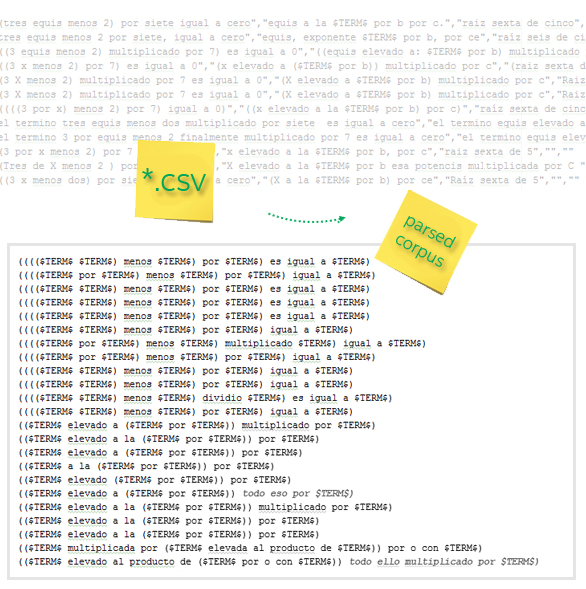
\includegraphics[width=11cm, height=11cm]{Figures/parsed_corpus}
  \caption[]{Funcionamiento de prepare\_corpus}
\label{fig:parsed_corpus}
\end{figure}

\subsection{Corpus building}

Esta parte del procedimiento se encarga de construir lo que será el corpus que se utilizará para hacer las evaluaciones de las transcripciones. En el corpus se reúne toda la información que los voluntarios dieron en su respuestas. Es información limpia y que puede exportarse para utilizarla en otro proyecto.

El comportamiento que describiré en esta sección puede encontrarse en el método \textbf{parse\_corpus} dentro de la misma clase.

Para crear el corpus simplemente se ha implementado un parser que sabe interpretar los datos limpios obtenidos por el punto anterior, para recolectar en un solo lado toda la información.

Este método se encarga de extraer de cada respuesta todas las estructuras gramaticales compuestas en él. Expliquemos esto mediante el siguiente ejemplo, supongamos:

\begin{tcolorbox}
input: ((\$TERM\$ elevado a (\$TERM\$ por \$TERM\$)) multiplicado por \$TERM\$)
output: []
\end{tcolorbox}

Nos posicionaremos entre el último paréntesis "(" y el primer paréntesis ")" a partir de él. Y extraemos eso como una regla gramatical atómica, reemplazandolo en la fórmula original como \$TERM\$.

\begin{tcolorbox}
input: ((\$TERM\$ elevado a \$TERM\$) multiplicado por \$TERM\$) \\
output: [(\$TERM\$ por \$TERM\$), ]
\end{tcolorbox}

Repetimos el algoritmo anterior obteniendo:

\begin{tcolorbox}
input: (\$TERM\$ multiplicado por \$TERM\$) \\
output: [(\$TERM\$ por \$TERM\$), (\$TERM\$ elevado a \$TERM\$)]
\end{tcolorbox}

El algoritmo finaliza cuando lo que encierran los paréntesis seleccionados es el total de la cadena. Por lo tanto el resultado que obtenemos es:

\begin{tcolorbox}
output: [(\$TERM\$ por \$TERM\$), (\$TERM\$ elevado a \$TERM\$), (\$TERM\$ multiplicado por \$TERM\$)]
\end{tcolorbox}

De esta manera pudimos extraer de una sola respuesta, gracias a tener los datos limpios, tres distintas reglas gramaticales que aportan a la construcción del evaluador final.

Finalmente, este proceso es aplicado a cada respuesta recibida obteniendo un abundante listado de reglas gramaticales que formarán parte de las evaluaciones.

\subsection{¿Cómo está organizado el corpus de reglas de gramaticales?}

Este corpus que reglas gramaticales, está compuesto por todas las reglas atómicas que se extrajeron en el procesamiento anterior. Cada regla gramatical denota una forma de escribir una sola operación matemática. Por ejemplo, si el operador en cuestión fuese la suma (que en MathML es tratado como plus) podemos obtener como reglas gramaticales atómicas los siguientes ejemplos \textbf{(\$VAR\$ sumado a \$VAR\$)} o \textbf{(\$VAR\$ mas \$VAR\$)} o aún así \textbf{(la suma de \$VAR\$ y \$VAR\$)}.

Luego, como paso final en todo este procesamiento. Para fines de performance, se busca persistir en un solo archivo información precalculada y necesaria para computar las evaluaciones.

Cada regla gramatical atómica está asociada a una etiqueta MathML que denote la relación directa entre la etiqueta y su verbalización. Dado que podemos tener distintas ocurrencias de la misma regla gramatical y la etiqueta, se decidió añadir a esta versión sumarizada del corpus un número que denote la cantidad de ocurrencias de una misma regla.

Por lo tanto, en conclusión, el siguiente es un extracto de este corpus mencionado:

\begin{tcolorbox}
root,42,(raiz \$TERM\$ de \$TERM\$)\\
function,70,(\$TERM\$ de \$TERM\$)\\
times,17,(\$TERM\$ multiplicado por \$TERM\$)\\
times,168,(\$TERM\$ por \$TERM\$)\\
exp,45,(\$TERM\$ al \$TERM\$)\\
exp,59,(\$TERM\$ a la \$TERM\$)
\end{tcolorbox}

Mediante él, podemos obtener respuestas a distintas preguntas que nos podamos hacer. Por ejemplo, ¿De cuántas maneras distintas regularmente se puede referir a la potencia?, ¿Qué regla es para la multiplicación es más frecuente?, ¿Hay alguna operación que se diga de la misma forma?.

\subsection{Constructor de evaluadores}

En el contexto de este trabajo final, una métrica es un indicador que evalúa la producción final o transcripción y representa la calidad de la salida.

La calidad de una traducción es inherentemente subjetiva, no hay ningún objetivo cuantificable o bueno. Por lo tanto, cualquier métrica debe asignar puntuaciones de calidad relacionadas con las que daría un humano. Es decir, una métrica debería puntuar alto a transcripciones que los humanos puntuen altamente, y dar puntuaciones bajas a aquellas que los humanos den puntuaciones bajas. El juicio humano es el punto de referencia para evaluar las métricas automáticas.

Este sistema define tres tipos de métricas que indicaran el grado de confianza que tendrá el usuario.\\

{\Large \textbf{Evaluador automático}}\\

Un evaluador automático es aquel que no necesita de la presencia de un humano para poder evaluar, es una métrica que se desarrolla y se ejecuta desatendidamente. Esta métrica se enfoca en medir \textbf{la fluidez de las transcripciones}.

Dado que para medir la fluidez no necesitamos conocer el lenguaje de origen (en el entorno de esta tesis serían las fórmulas matemáticas) y si conocer el lenguaje destino (transcripciones) esta métrica es desarrollada y ejecutada gracias a la presencia de los datos recolectados con las encuestas.

Por cada transcripción que el usuario consulte, se le informará el grado de confianza de esa transcripción. Para ayudarnos a entender qué significa el grado de confianza, enunciaré algunas definiciones.\\

\textbf{Definición:}\\El \textit{\textbf{conjunto de las transcripciones atómicas}, es el conjunto de todas las reglas gramaticales atómicas que llevaron a producir la transcripción.}
Por ejemplo:\\
Para el caso de $x^{ab}$ tenemos que su transcripción asociada es: \textit{(X elevado a la (A multiplicado por B))} entonces el conjunto de las transcripciones atómicas es el conjunto que contiene a \$TERM\$ multiplicado por \$TERM\$) y (\$TERM\$ elevado a la \$TERM\$). Dado que solo ambas reglas gramaticales han sido usadas para producir la transcripción.\\

\textbf{Definición:}\\\textit{La \textbf{etiqueta asociada a una transcripción}, denotada como $tag(t_i)$, es la etiqueta MathML para la cual tiene asociada tal transcripción atómica.\\Para el caso de (\$TERM\$ mas \$TERM\$) el tag asociado es \textbf{plus}.}\\

Con estas definiciones estamos listos para definir la métrica que queremos mencionar.

\textbf{Definición:}\\Sea trx una transcripción obtenida por el verbalizador, se define como \textbf{grado de confianza} a:

$$GDC(trx) = \prod_{t_i \in trx} \frac{count(t_i)}{count(tag(t_i))}$$

Dónde se denota $t_i$ como las transcripciones atómicas dentro de $trx$.\\
$count(t_i)$ es la cantidad de ocurrencias de la $t_i$ en el corpus sumarizado.\\
$count(tag(t_i))$ es la cantidad de transcripciones que tiene el tag asociado a la $t_i$.

Esta métrica es un número entre 0 y 1, que intenta mostrarle al usuario un número que represente que tan frecuente es la transcripción con respecto a los datos obtenidos por los usuarios mediante los formularios.

Dado que todos los datos que el cálculo de GDC pide están presentes en el corpus de información externa, hace que esta métrica pueda ser calculada automáticamente.

Actualmente TexToES está mostrando por cada transcripción su versión percentil de la métrica $(GDC(trx) * 100)$

\begin{figure}[H]
\centering
  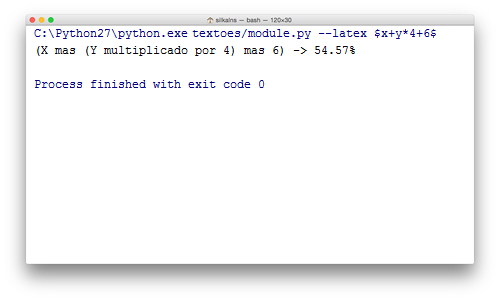
\includegraphics[width=11cm, height=6.62cm]{Figures/demo_1}
  \caption[]{GDC de una transcripción}
\label{fig:demo_1}
\end{figure}

{\Large \textbf{Evaluador semi-automático (human-in-the-loop)}}\\

Este tipo de evaluadores semi-automáticos (HITL o human-in-the-loop\cite{9}) son evaluadores que requieren la interacción del humano para poder proceder.

La idea detrás de este método es ver si los usuarios de TexToES podrían interpretar y reconstruir la fórmula original que ha sido el input de una verbalización; en analogía con la traducción automática, esto correspondería a evaluar TexToES mediante la retrotraducción o traducción inversa; esta evaluación permite medir la adecuación o fidelidad de la traducción. El procedimiento fue el siguiente:

\begin{itemize}
   \item Se han seleccionado 20 fórmulas latex y se ha estimulado TexToES con ellas obteniendo 20 transcripciones.
   \item Se ha construido una encuesta con estas 20 transcripciones y se les ha pedido a voluntarios que escriban la fórmula matemática asociada a esa transcripción.
   \item Por cada respuesta, se ha reconstruido la fórmula latex.
   \item Se compara de igual a igual las fórmulas latex obtenidas con las fórmulas latex empleadas para obtener las transcripciones
\end{itemize}

Los datos empleados (latex y transcripción) en la encuesta pueden ser encontrados en el Apéndice de esta tesis, como así también las respuestas de los voluntarios.

Esta es la parte donde el humano participa en la evaluación, el resto de la evaluación es automática pero necesita de recolectar resultados a través de humanos.

Por lo tanto queremos ver cómo se comporta TexToES informando una transcripción, vamos a definir para este tipo de evaluación la siguiente métrica GDC.

$$GDC = \sum_{i=1}^{N} \frac{1}{N^2}*count(latex_i==resp_i)$$

Dónde N es la cantidad de transcripciones evaluadas, en este caso fueron 13.\\
$latex_i$ es el i-ésimo latex empleado para obtener la transcripción.\\
$resp_i$ es la respuesta i-ésima (que también es un latex) por parte de los voluntarios.

Cabe mencionar que esta métrica de confianza no es una métrica que habla de una transcripción, sino más bien es una métrica que habla de la confianza del sistema de traducción. La métrica intenta capturar la idea de la proporción de un promedio de respuestas correctas.\\

{\Large \textbf{Evaluador humano}}\\

Se han presentados dos evaluadores que buscan definir la calidad de la transcripción pero, sin embargo, la calidad de la traducción es algo subjetivo y de cierta manera el Gold Standard es tener un juicio humano sobre nuestro sistema. Dado que la salida de este sistema es para un ser humano, es correcto pensar que un ser humano lo evalúe. Por otro lado, en la instancia de evaluación humana están presentes factores propias de la comprensión que le permite al juez identificar posibles errores en la traducción.

Pero para ello se necesita de tener un juez humano que entienda tanto del tipo de entrada (\textbf{source}) como el tipo de salida (\textbf{target}) para poder hacer el juicio subjetivo sobre la traducción, esto implica hacer un juicio subjetivo indicando la calidad de una transcripción para una fórmula matemática dada.

La técnica empleada de medición aquí fue presentar una serie de fórmulas matemáticas con sus respectivas transcripciones y se le pide al juez calificar utilizando una escala de múltiples puntos. Estas calificaciones requiere de un juez que entienda ambos lenguajes.

El juicio puesto en juego es de si \textbf{la transcripción es adecuada para la fórmula}.

Se ha utilizado Google Forms para hacer estas preguntas a los voluntarios, presentando las fórmulas con sus verbalizaciones, y una escala tipo Likert\cite{12} para que indiquen su juicio al respecto.

\begin{figure}[H]
\centering
  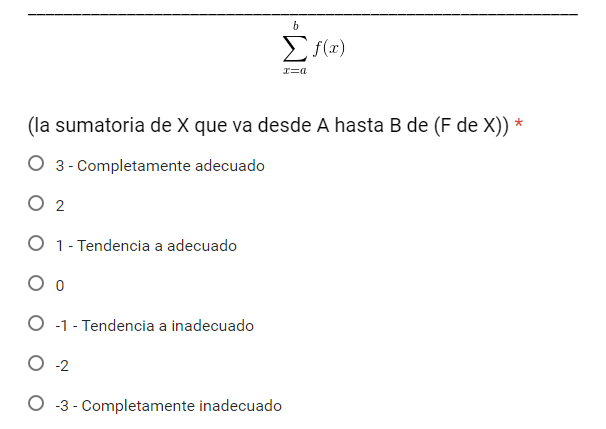
\includegraphics[width=11cm, height=6.62cm]{Figures/evaluadorhumano}
  \caption[]{Evaluador humano}
\label{fig:evaluadorhumano}
\end{figure}

Se han escrito un total de 20 preguntas que muestran las fórmulas matemáticas en imágenes junto a las transcripciones obtenidas con TexToES. Las 20 fórmulas matemáticas intentan contener todo el alcance de TexToES desde sumas, restas hasta sumatorias y aplicación de funciones, y sus combinaciones.

Los resultados obtenidos se muestran en la siguiente sección.


\subsection{Recolección de resultados}

Hemos mostrado varias formas de medir TexToES que buscan estar alineados con el juicio humano, es decir, si un humano dice que la transcripción es buena queremos que nuestros evaluadores digan lo mismo, y así también con los casos en que las transcripciones sean malas. En esta sección se intenta enumerar algunos resultados obtenidos para intentar aplicar correcciones a TexToES para volverlo más natural.

De los tres tipos de métricas que se han elaborado pudimos extraer sugerencias y conocer cómo es que el usuario final suele leer las distintas fórmulas matemáticas.

Para el caso de las encuestas que sirvieron para evaluar las transcripciones automáticamente, aquellas que se le pedía al voluntario cómo leerían un conjunto de fórmulas matemáticas, se han extraído los siguientes patrones.\\

{\Large \textbf{Patrones de traducción}}\\

\begin{itemize}

   \item El 100\% de los encuestados se refiere a la suma entre x e y como \textbf{X más Y}. Por lo tanto la regla de traducción para la etiqueta <plus> debería ser completada con la regla mencionada.
   \item Tanto para el caso de la potencia como para la raíz, el 100\% de los encuestados utilizan \textbf{cuadrado} y \textbf{cubo} para referirse a la aplicación de esas funciones para el 2 y el 3 respectivamente.
   \item Cuando no es la raíz cuadrada ni cúbica, el 100\% de los encuestados utiliza \textbf{raiz X de Y}.
   \item Cuando no es la exponente cuadrada ni cúbica, el 41\% de los encuestados se refiere a \textbf{X a la Y} para mencionar el operador exponencial de X con Y. El 33\% lo menciona como \textbf{X al Y} y el 26\% lo menciona como \textbf{X elevado a Y}
   \item Así como a la suma, para el caso de la resta el 100\% de los encuestados dicen \textbf{X menos Y}.
   \item El 55\% de los encuestados igualan x con y mencionando \textbf{X es igual a Y}, mientras que el resto dicen \textbf{X igual a Y}.
   \item Para el caso de la multiplicación tenemos que el 90\% se refiere a la multiplicación entre x con y como \textbf{X por Y}, mientras que el 10\% restante lo dice como \textbf{X multiplicado por Y}. Es importante notar aquí que TexToES prefiere traducir la multiplicación como\textit{ X multiplicado por Y} haciendo que elija la transcripción menos probable. Una acción a tomar a partir de aquí es cambiar la regla de traducción de TexToES para que elija la más probable.
   \item El 73\% de los encuestados se refieren a la división entre x e y como \textbf{X sobre Y}, mientras que el porcentaje restante elige decir \textbf{X dividido Y}. Cambiar la regla de traducción de TexToES para este caso también hará cambiar las métricas.

\end{itemize}

Estos son algunos datos que podemos extraer de las encuestas realizadas para evaluar a TexToES automáticamente.\\

Algunas sugerencias por partes de los humanos entrevistados para el evaluador semiautomático fueron:
\begin{itemize}
\item Utilizar \textbf{A intersección B}, en lugar de \textbf{A intersectado por el conjunto B} para el caso de la intersección entre dos conjuntos.
\item En la aplicación de la función F en el argumento X, mencionar \textbf{F de X} en lugar de \textbf{F evaluado en X}.
\end{itemize}

Es importante mencionar que estas sugerencias fueron tomadas para modificar la forma de traducir de TexToES, dado que coinciden con la extracción de patrones detalladas en el punto anterior.

Por último, por el lado de la evaluación con juicio humano presentaré aquí algunos resultados.

En total se han recibido una cantidad de \textbf{29 respuestas} para las 20 preguntas que presentaba el Formulario.

Recordemos que cada juez voluntario podía evaluar la transcripción puntuando de la siguiente manera

\begin{itemize}
   \item \textbf{3} \textit{completamente adecuado}
   \item \textbf{2}
   \item \textbf{1} \textit{tendencia a adecuado}
   \item \textbf{0}
   \item \textbf{-1} \textit{tendencia a inadecuado}
   \item \textbf{-2}
   \item \textbf{-3} \textit{completamente inadecuado}
\end{itemize}

Para ayudarnos a interpretar algunos resultados vamos a dividir la tabla de puntos anteriores en tres categorías. La categoría que contiene los puntajes 3, 2 y 1 serán llamados puntajes \textbf{buenos}, para los puntajes marcados como 0 será tratado como puntaje \textbf{neutro} finalmente, para los puntajes de -1, -2 y -3 serán llamados puntajes \textbf{malos}.
Algunos datos interesantes que pueden observarse son:

\begin{itemize}
   \item 9 de 20 transcripciones obtuvieron un puntaje de 3 (completamente adecuado) con más del 70\%
   \item Solo 2 de 20 transcripciones obtuvieron un puntaje entre -3 y -2, y lo obtuvieron como 5\%
   \item 9 de 20 transcripciones obtuvieron solo puntajes buenos
   \item 20 de 20 transcripciones obtuvieron en su mayoría de respuestas puntajes buenos
\end{itemize}

Podemos observar, con la siguiente imagen, que solo una transcripción de las 20 ha obtenido 3 como puntaje en todas sus respuestas asociadas.

\begin{figure}[H]
\centering
  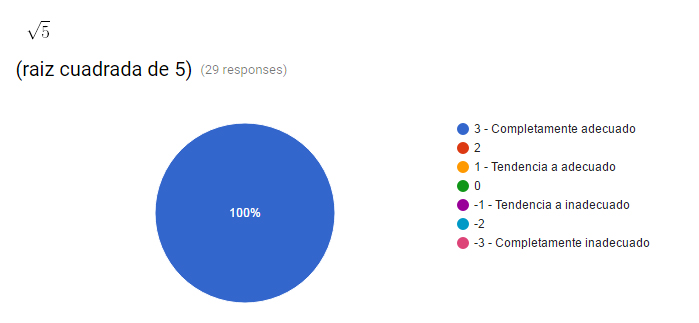
\includegraphics[width=15cm, height=6.93cm]{Figures/captura2}
  \caption[]{Transcripción con 100\% de respuestas en completamente adecuado}
\label{fig:captura2}
\end{figure}

El siguiente es un ejemplo de las 9 transcripciones que ha recibido solo puntaje bueno. Como se puede observar el 100 \% de sus respuestas están en el conjunto de calificaciones buenas (1, 2 o 3)

\begin{figure}[H]
\centering
  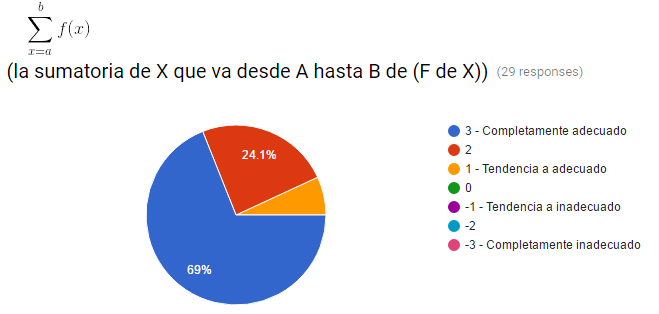
\includegraphics[width=15cm, height=7.15cm]{Figures/captura1}
  \caption[]{Transcripción con solo puntaje bueno}
\label{fig:captura1}
\end{figure}

Y por último, el siguiente es el caso que más respuestas variadas ha tenido y aún así en su mayoría ha obtenido un puntaje bueno. El 69 \% de sus respuestas han incluido 1, 2 y 3 como calificación. Además este también es 1 de las 2 transcripciones que ha obtenido un 3 en el 5\% del total de sus calificaciones.

\begin{figure}[H]
\centering
  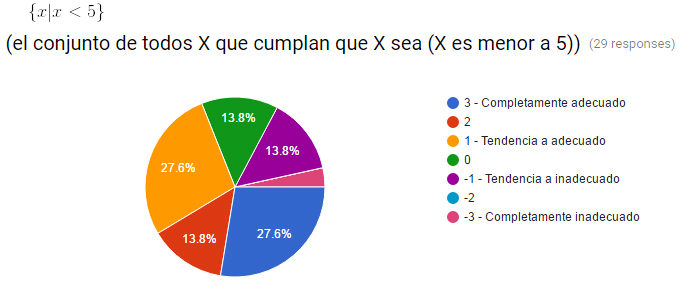
\includegraphics[width=15cm, height=6.39cm]{Figures/captura3}
  \caption[]{Transcripcion con solo puntaje bueno}
\label{fig:captura3}
\end{figure}

Usted puede consultar la lista completa de respuestas en el anexo de este documento. 
%\chapter{Discusión general}

\label{Chapter5}

\section{Fortalezas y limitaciones}
TexToES es un \textbf{prototipo} o \textbf{prueba de concepto} que nos ayuda a resolver el problema de accesibilidad que planteamos en los primeros capítulos pero, sin embargo, no es una solución definitiva.

Hay un amplio rango de operaciones matemáticas que TexToES no cubre. Recordemos que TexToES tiene una dependencia con un componente externo, que es SnuggleTeX. Resulta que, dada esa dependencia, TexToES manipula el CMathML devuelto por SnuggleTeX, entonces para todos los casos que SnuggleTeX no tenga una respuesta que dar TexToES no podrá traducir. A su vez, no solo heredaremos la funcionalidad de SnuggleTeX sino también sus errores.

Por ejemplo, SnuggleTeX trata toda variable i como un número imaginario, lo que a primera medida parece ser correcto luego vemos que no lo es. Si queremos que trate como número imaginario la siguiente expresión

$$2i + 3$$

pero, sin embargo, no queremos que lo haga con los subíndices ya que en éste contexto es incorrecto.

$$x_i$$

Por otro lado, TexToES se ha construído asumiendo que la traducción de LaTeX a Español cumple con una relación directa de uno a uno. Donde cada operacion LaTeX se corresponde con un fraseo al español. Esta es una asunción que nos ayuda a resolver el problema, pero que no es una solución completa.

Si bien, podemos siempre devolver la transcripción más probable para cada operación no es correcto pensar que la transcripción final es la más probable.

Por ejemplo, prestemos atención a la siguiente fórmula matemática:

$$ (3x + 2) y $$

Podemos ver, gracias a los resultados obtenidos de los contribuyentes, que para la multiplicación la transcripción más frecuente es \$TERM\$ por \$TERM\$. Entonces TexToES procesará aquella expresión y devolverá como transcripción \textbf{\textit{((3 por X mas 2) por Y)}}, lo cual es correcto. Pero se ha descubierto que para estos patrones donde hay más de una multiplicación se tiende a decir \textbf{todo eso multiplicado por} para las multiplicaciones en la cual uno de sus operandos es una combinación de otras operaciones (resultando: \textbf{\textit{((3 por X mas 2) todo eso multiplicado por Y)}}). TexToES, con la implementación actual, no puede capturar este comportamiento.

\section{Trabajo futuro}

Aquí se listan los posibles lineamientos a seguir si se decidiese continuar con éste proyecto.\\

{\Large \textbf{Interfaz gráfica y lector}}

Una arista a encarar puede ser prestarle atención al ScreenReader que se utilizará para leer ésto. Quizás se puede dejar de asumir que el usuario utilizará su preferido, y se podría extender TexToES añadiendo un sistema TTS que añada las pausas necesarias y velocidades para ayudar al usuario final a entender mejor la fórmula\\

{\Large \textbf{Independencia a SnuggleTeX}}

SnuggleTeX fue un producto desarrollado para alcanzar un doctorado y lleva 8 años sin mantenimiento. Quizás un posible trabajo a futuro sea desarrollar un \textbf{convertidor de LaTeX a CMathML} de los operadores más utilizados para el público que se desea apuntar. Esto ayudaría a eliminar la dependencia con esta librería, y ayudaría a mitigar errores.\\

{\Large \textbf{Extender SnuggleTeX}}

Si desarrollar una aplicación similar a SnuggleTeX que obtenga CMathML a partir de LaTeX no es factible, probablemente extender SnuggleTeX sea una opción. Un aporte a este producto seguramente ayudará a otros desarrolladores que se encuentren usando actualmente el producto. El lineamiento aquí es extender SnuggleTeX con los operadores que SnuggleTeX no soporta.\\

{\Large\textbf{ Modelo de lenguaje}}

Con un modelo de lenguaje se puede resolver el problema de capturar siempre la transcripción más probable o frecuente para una fórmula LaTeX dada. Se puede pensar en ir obteniendo las transcripciones más frecuentes basadas en un análisis de N-Gramas. Esto hará que, para el ejemplo citado arriba, si uno de los operandos de la multiplicación es extenso u obtiene una combinación de otras operaciones entonces opte por la transcripción \textbf{todo eso multiplicado por}. 

%----------------------------------------------------------------------------------------
%	THESIS CONTENT - APPENDICES
%----------------------------------------------------------------------------------------

\appendix % Cue to tell LaTeX that the following "chapters" are Appendices

% Include the appendices of the thesis as separate files from the Appendices folder
% Uncomment the lines as you write the Appendices

\chapter{Acerca de la implementación de TexToES}

\label{AppendixA}

TexToES fue programado con Python 2.7.9 y con la ayuda de librerias como xml.etree, ConfigObj y request. Cada una de las tres librerías pueden instalarse con pip.
A continuación se lista la organización del directorio que contiene la solución.

\begin{lstlisting}[basicstyle=\scriptsize]
+ TexToES
  | corpus
  + - forms_data
    - hitl_responses
    - hjudgement
    - corpus.txt
    - parsed_responses.txt
    - summarized_corpus.txt
  | tesis_document_sourcecode
  + - Appendices
    - Chapters
    - Figures
    - TexToES - Thur Luis - Trabajo Final.pdf
    - TexToES - Thur Luis - Trabajo Final.tex
  + evidencia.txt
  + language.template
  + lenguage_evaluator.py
  + lenguage_generator.py
  + LICENCE
  + mathml_client.py
  + module.py
  + preprocessor.py
  + test_module.py
\end{lstlisting}

La carpeta \textbf{corpus} contiene lo necesario para evaluar la transcripcion, dentro contiene los siguientes elementos:
\begin{itemize}
\item forms\_data: Contiene los archivos CSV con las respuestas de los voluntarios que contestaron como leerian las formulas matematicas.
\item hitl\_responses: Contiene los archivos CSV con las respuestas de los voluntarios que participaron en la evaluacion de retrotraduccion
\item hjudgement: Contiene los archivos CSV con las respuestas de los jueces  que evaluaron las transcripciones de TexToES
\item corpus.txt: Archivo que contiene todas las reglas gramaticales atomicas presentes en los archivos .CSV en forms\_data
\item parsed\_responses.txt: Contiene todas las respuestas CSV en forms\_data procesadas
\item summarized\_corpus.txt: Contiene las ocurrencias de reglas gramaticales atomicas con la correspondencia anotada de la etiqueta CMathML a la cual se relaciona
\end{itemize}

También tenemos una carpeta donde se encuentra todo el código usado para generar el pdf de éste documento, puede ser encontrado en textbf{tesis\_document\_sourcecode}, ésta contiene los siguientes elementos:
\begin{itemize}
\item Appendices: Apendices de la tesis
\item Chapters: Capitulos de la tesis
\item Figures: Figuras de la tesis
\item TexToES - Thur Luis - Trabajo Final.pdf: Documento principal de tesis en formato pdf.
\item TexToES - Thur Luis - Trabajo Final.tex: Documento principal de tesis en format tex para editar.
\end{itemize}

Finalmente, en la carpeta raíz tenemos los siguientes elementos.

\begin{itemize}
\item evidencia.txt: Aqui se listan todas las transcripciones que TexToES ha hecho desde el inicio, sirve para regresionar sobre TexToES cuando alguna funcionalidad nueva se agrega.
\item test\_module.py: Modulo de testing para regresionar.
\item module.py: Modulo principal de TexToES, se utiliza para obtener la transcripcion para una expresion matematica.
\item mathml\_client.py: Cliente que se comunica con SnuggleTeX, es alimentado por module.py si vino como entrada un string latex. Obtiene el CMathML asociado, y alimenta a preprocessor.py
\item preprocessor.py: Dada una formula matematica CMathML va a generar el stack que luego alimentará a lenguage\_generator.py para ir obteniendo las traducciones.
\item lenguage\_generator.py: Se encarga de traducir las partes mas atomicas de la expresion matematica, procesa el stack que recibe de preprocessor.py
\item language.template: Contiene todas las reglas de transcripciones, usadas por language\_generator.py
\item lenguage\_evaluator.py: Se encarga de darle un puntaje a las transcripciones basado en los datos que hay en forms\_data
\item LICENCE, licencia de TexToES
\end{itemize}

Aqui podemos observar el diagrama de clases de la implementación de TexToES.

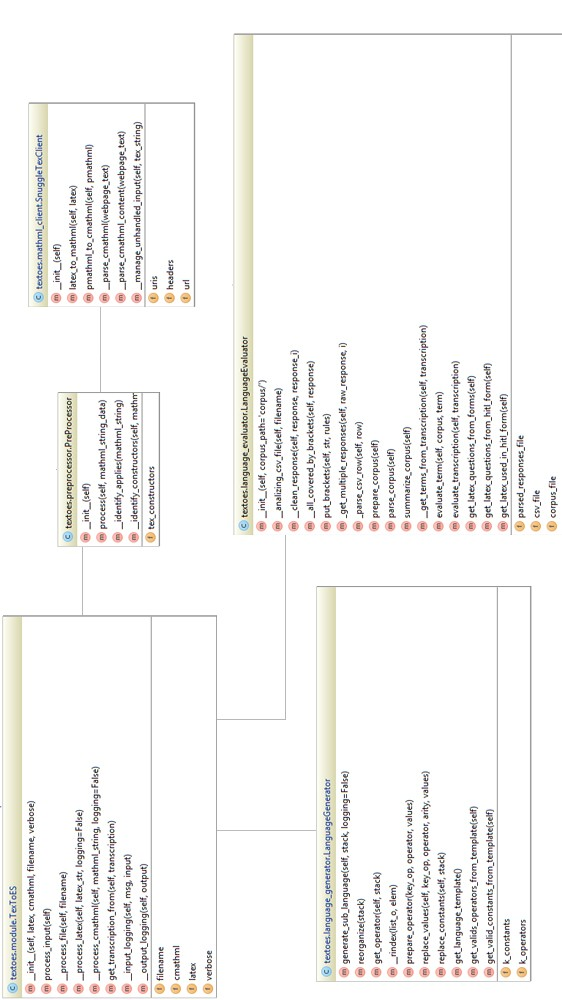
\includegraphics[width=11.24cm, height=20cm]{figures/diagram.jpg}

Finalmente, usted puede consultar el código fuente en GitHub\footnote{https://github.com/lthurr/textoes}. Los comentarios inline en el código puede ayudarle a entender mucho mejor la implementación.

%\chapter{Reglas de transcripción}

\label{AppendixB}

En este apéndice se listan todas las reglas de transcripción que TexToES usa para poder obtener una transcripción final.

Del lado izquierdo esta la etiqueta CMathML que representa la entidad matemática mientras que del lado derecho está la transcripción.

\begin{lstlisting}[basicstyle=\scriptsize]
[constantes]
  infinity = infinito
  imaginaryi = I
  integers = conjunto de los enteros
  emptyset = conjunto vacio
  real = el conjunto de los reales

[operadores]
#Constructores
  list = la lista de $VAR$
  vector = el vector compuesto por $VAR$
  set = el conjunto de todos $VAR$ que cumplan que
    $bvar$ sea $condition$, el conjunto de $VAR$
  imaginary = Operacion imaginaria $VAR$

#Relaciones
  eq = $VAR$ es igual a $VAR$
  neq = $VAR$ no es igual a $VAR$
  gt = $VAR$ es mayor a $VAR$
  geq = $VAR$ es mayor o igual a $VAR$
  lt = $VAR$ es menor a $VAR$
  leq = $VAR$ es menor o igual a $VAR$
  equivalent = $VAR$ es equivalente a $VAR$
  approx = $VAR$ es aproximado a $VAR$
  factorof = $VAR$ divide a $VAR$

#Operadores basicos
  plus = $VAR$ mas $VAR$
  minus = $VAR$ menos $VAR$, menos $VAR$
  times = $VAR$ por $VAR$
  divide = $VAR$ dividido $VAR$
  power = $VAR$ elevado a la $VAR$
  exp = e elevado a la $VAR$
  root = raiz $degree$ de $VAR$

#Calculo
  sum = la sumatoria de $bvar$ que va desde
    $lowlimit$ hasta $uplimit$ de $VAR$
  product = la productoria de $bvar$ que
    va desde $lowlimit$ hasta $uplimit$ de $VAR$
  limit = el limite de $bvar$ que tiende
    $lowlimit$ de $VAR$

#Operadores logicos
  not = $VAR$ negado
  and = $VAR$ y $VAR$
  or = $VAR$ o $VAR$
  implies = $VAR$ implica $VAR$

#Conjuntos
  in = $VAR$ en $VAR$
  notin = $VAR$ no esta en $VAR$
  intersect = $VAR$ intersectado con el conjunto $VAR$
  union = $VAR$ union $VAR$
  setdiff = $VAR$ menos el conjunto $VAR$
  prsubset = $VAR$ es subconjunto de $VAR$

#Funciones conocidas
  function = $VAR$ de $VAR$
  inverse = $VAR$ inversa
  max = maximo entre $VAR$
  determinant = determinante de $VAR$
  gcd = maximo comun divisor entre $VAR$ y $VAR$
  lcm = minimo comun multiplo entre $VAR$ y $VAR$
  factorial = $VAR$ factorial
  ln = logaritmo natural de $VAR$
  log = logaritmo $base$ de $VAR$
  sin = seno de $VAR$
  arcsin = arcoseno de $VAR$
  cos = coseno de $VAR$
  arccos = arcocoseno de $VAR$
  tan = tangente de $VAR$
  arctan = arcotangente de $VAR$
  sinh = seno hiperbolico de $VAR$
  arcsinh = arcoseno hiperbolico de $VAR$
  cosh = coseno hiperbolico de $VAR$
  arccosh = arcocoseno hiperbolico de $VAR$
  tanh = tangente hiperbolica de $VAR$
  arctanh = arcotangente hiperbolica de $VAR$
  sech = secante hiperbolica de $VAR$
  arcsech = arcosecante hiperbolica de $VAR$
  csch = cosecante hiperbolica de $VAR$
  arccsch = arcocosecante hiperbolica de $VAR$
  coth = cotangente hiperbolica de $VAR$
  arccoth = arcocotangente hiperbolica de $VAR$
  cot = cotangente de $VAR$
\end{lstlisting}

%\chapter{Resultados de retrotraducción}

\label{AppendixC}

Aquí se listan las transcripciones usadas en el proceso de evaluación mediante la retrotraducción.
Del lado derecho de la tabla usted puede ver el latex utilizado para generar las transcripciones que estan en el lado izquierdo.

\begin{center}
 \begin{tabular}{||c  c||}
    \hline
    Transcripción & LaTeX usado \\ [0.5ex]
    \hline\hline
    (raiz 6 de 5) & $\sqrt[6]{5}$ \\ 
    \hline
    (X elevado a la (1 dividido 2))& $x^\frac{1}{2}$ \\
    \hline
    (A no esta en conjunto vacio)& $a \not\in \emptyset$ \\
    \hline
    (A union B)& $A \cup B$ \\
    \hline
    ((1 es menor o igual a X) y (X es menor a Y))& $1\leq x < y$ \\
    \hline
    (conjunto de los enteros no es igual a conjunto vacio)& $\mathbb{Z} \neq \emptyset$ \\
    \hline
    ((seno de X) mas (logaritmo natural de Y) mas (cotangente de Z))& $\sin x + \ln y + \cot z$ \\
    \hline
    (((3 multiplicado por X) menos 7) es igual a 0)& $3x - 7 = 0$ \\
    \hline
    (A multiplicado por B)& $A \times B$ \\
    \hline
    (A no es igual a B)& $A \neq B$ \\
    \hline
    (A intersectado con el conjunto B)& $A \cap B$ \\
    \hline
    (((P negado) negado) es igual a P)& $\lnot \lnot p = p$ \\
    \hline
    (1 dividido (3 mas 7))& $\frac{1}{3+7}$ \\
    \hline
    ((F aplicado a X) es igual a (X elevado a la 3)) & $f(x) = x^3$ \\[1ex]
 \hline
\end{tabular}
\end{center}

Recordemos que el objetivo de esta evaluación era pedirles a los voluntarios que escribieran la fórmula que les sugería la transcripción para luego compararlas con las fórmulas reales usadas.

Las respuestas en las siguientes tablas, $t_i$ significa la transcripción i, $v_i$ significa el voluntario i.

\begin{center}
\begin{tabular}{ |c|c|c|c|c|c|c|c| }
 \hline
    $v$ & $t_1$ & $t_2$ & $t_3$ & $t_4$ & $t_5$ & $t_6$ & $t_7$ \\[0.5ex]
    \hline\hline
    $v_1$ & $ \sqrt[6]{5}$ & $x^\frac{1}{2}$ & $a \not\in \emptyset$          & $A \cup B$ & $1\leq x \wedge x < y$    & $\mathbb{Z} \neq \emptyset$            & $\sin x + \ln y + \cot z$  \\
    $v_2$ &$ \sqrt[6]{5}$ & $x^\frac{1}{2}$ & $a \not\in \emptyset$          & $A \cup B$ & $1\leq x < y$             & $\{ \mathbb{Z} \} \neq \emptyset$      & $\sin x + \ln y + \cot z$  \\
    $v_3$ &$ \sqrt[6]{5}$ & $x^\frac{1}{2}$ & $a \not\in \emptyset$          & $A \cup B$ & $1\leq x \wedge x < y$    & $\{ \mathbb{Z} \} \neq \{\emptyset\}$  & $\sin x + \ln y + \cot z$  \\
    $v_4$ &$ \sqrt[6]{5}$ & $ \sqrt{2}$     & $a \not\in \emptyset$          & $A \cup B$ & $1\leq x \wedge x \leq y$ & $\mathbb{Z} \neq \emptyset$            & $\sin x + \ln y + \cot z$  \\
    $v_5$ &$ \sqrt[6]{5}$ & $x^{1 \div 2}$  & $a \not\in \left \{ \right \}$ & $A \cup B$ & $1\leq x \wedge x < y$    & $\mathbb{Z} \neq \left \{ \right \}$   & $\sin x + \ln y + \cot z$  \\
    $v_6$ &$ \sqrt[6]{5}$ & $x^\frac{1}{2}$ & $a \not\in \emptyset$          & $A \cup B$ & $1\leq x \wedge x < y$    & $\mathbb{Z} \neq \emptyset$            & $\sin x + \ln y + \cot z$  \\
    $v_7$ &$ \sqrt[6]{5}$ & $x^\frac{1}{2}$ & $a \not\in \emptyset$          & $A \cup B$ & $1\leq x \wedge x < y$    & $\mathbb{Z} \neq \emptyset$            & $\sin x + \ln y + \cot z$  \\
    $v_8$ &$ \sqrt[6]{5}$ & $x^\frac{1}{2}$ & $a \not\in \emptyset$          & $A \cup B$ & $1\leq x \wedge x < y$    & $\mathbb{Z} \neq \emptyset$            & $\sin x + \ln y + \cot z$  \\
    $v_9$ &$ \sqrt[6]{5}$ & $x^\frac{1}{2}$ & $a \not\in \emptyset$          & $A \cup B$ & $1\leq x \wedge x < y$    & $\mathbb{Z} \neq \emptyset$            & $\sin x + \ln y + \cot z$  \\
    $v_{10}$ &$ \sqrt[6]{5}$ & $x^\frac{1}{2}$ & $a \not\in \emptyset$          & $A \cup B$ & $1\leq x \wedge x > y$    & $\mathbb{Z} \neq \emptyset$            & $\sin x + \ln y + \cot z$  \\
    $v_{11}$ &$ \sqrt[6]{5}$ & $x^\frac{1}{2}$ & $a \not\in \emptyset$          & $A \cup B$ & $1\leq x \wedge x > y$    & $\mathbb{Z} \neq \emptyset$            & $\sin x + \ln y + \cot z$  \\
    $v_{12}$ &$ \sqrt[6]{5}$ & $x^\frac{1}{2}$ & $a \not\in \emptyset$          & $A \cup B$ & $1\leq x \wedge x > y$    & $\mathbb{Z} \neq \emptyset$            & $\sin x + \ln y + \cot z$  \\
    $v_{13}$ &$ \sqrt[6]{5}$ & $x^\frac{1}{2}$ & $a \not\in \{\emptyset\}$      & $A \cup B$ & $1\leq x \wedge x < y$    & $\mathbb{Z} \neq \emptyset$            & $\sin x + \ln y + \cot z$  \\
 \hline
\end{tabular}
\end{center}


\begin{center}
\begin{tabular}{ |c|c|c|c|c|c|c|c| }
 \hline
 $v$ & $t_8$        & $t_9$        & $t_10$     & $t_11$     & $t_12$              & $t_13$          & $t_14$ \\[0.5ex]
    \hline\hline
 $v_1$ & $3x - 7 = 0$ & $A \times B$ & $A \neq B$ & $A \cap B$ & $\lnot \lnot p = p$ & $\frac{1}{3+7}$ & $f(x) = x^3$ \\
 $v_2$ & $3x - 7 = 0$ & $A \times B$ & $A \neq B$ & $A \cap B$ & $\lnot \lnot p = p$ & $\frac{1}{3+7}$ & $f(x) = x^3$ \\
 $v_3$ & $3x - 7 = 0$ & $A \times B$ & $A \neq B$ & $A \cap B$ & $\lnot \lnot p = p$ & $\frac{1}{3+7}$ & $f(x) = x^3$ \\
 $v_4$ & $3x - 7 = 0$ & $A \times B$ & $A \neq B$ & $A \cap B$ & $\lnot \lnot p = p$ & $1\div(3+7)$    & $f(x) = x^3$ \\
 $v_5$ & $$           & $A \times B$ & $A \neq B$ & $A \cap B$ & $\lnot \lnot p = p$ & $1 \div (3+7)$  & $f(x) = x^3$ \\
 $v_6$ & $3x - 7 = 0$ & $A \times B$ & $A \neq B$ & $A \cap B$ & $\lnot \lnot p = p$ & $\frac{1}{3+7}$ & $f(x) = x^3$ \\
 $v_7$ & $3x - 7 = 0$ & $A \times B$ & $A \neq B$ & $A \cap B$ & $\lnot \lnot p = p$ & $\frac{1}{3+7}$ & $f(x) = x^3$ \\
 $v_8$ & $3x - 7 = 0$ & $A \times B$ & $A \neq B$ & $A \cap B$ & $\lnot \lnot p = p$ & $\frac{1}{3+7}$ & $f(x) = x^3$ \\
 $v_9$ & $3x - 7 = 0$ & $A \times B$ & $A \neq B$ & $A \cap B$ & $\lnot \lnot p = p$ & $\frac{1}{3+7}$ & $f(x) = x^3$ \\
 $v_{10}$ & $3x - 7 = 0$ & $A \times B$ & $A \neq B$ & $A \cap B$ & $\lnot \lnot p = p$ & $\frac{1}{3+7}$ & $f(x) = x^3$ \\
 $v_{11}$ & $3x - 7 = 0$ & $A \times B$ & $A \neq B$ & $A \cap B$ & $\lnot \lnot p = p$ & $\frac{1}{3+7}$ & $f(x) = x^3$ \\
 $v_{12}$ & $3x - 7 = 0$ & $A \times B$ & $A \neq B$ & $A \cap B$ & $\lnot \lnot p = p$ & $\frac{1}{3+7}$ & $f(x) = x^3$ \\
 $v_{13}$ & $3x - 7 = 0$ & $A \times B$ & $A \neq B$ & $A \cap B$ & $\lnot \lnot p = p$ & $\frac{1}{3+7}$ & $f(x) = x^3$ \\
 \hline
\end{tabular}
\end{center}



%----------------------------------------------------------------------------------------
%	BIBLIOGRAPHY
%----------------------------------------------------------------------------------------
\renewcommand{\bibname}{Referencias}
\begin{thebibliography}{99}

\bibitem{censo}
Censo Nacional de Población,
Hogares y Viviendas 2010
Instituto Nacional de Estadística y Censos, Argentina
Disponible: \url{http://www.indec.gov.ar/ftp/cuadros/sociedad/PDLP_10_14.pdf}

\bibitem{w3MathML}
Mathematical Markup Language (MathML) Version 3.0 2nd Edition
1998-2014 W3C (MIT, ERCIM, Keio, Beihang)
\url{https://www.w3.org/TR/MathML3/}

\bibitem{SnuggleTeX}
SnuggleTeX (1.2.2), David McKain
University of Edinburgh
\url{http://www2.ph.ed.ac.uk/snuggletex/documentation/generating-content-mathml.html}

\bibitem{STClient}
SnuggleText - DEMO
Disponible: \url{http://www2.ph.ed.ac.uk/snuggletex/UpConversionDemo}

\bibitem{Relacion}
Recurso online donde muestra la relacion entre MathML y TEX
Disponible: \url{http://tex.stackexchange.com/questions/57717/relationship-between-mathml-and-tex}

\bibitem{MathAssesor}
The Wikipedia Math Accessor
Leo Ferres
University of Concepcion, Chile, 2006,
Disponible: \url{http://www.inf.udec.cl/~josefuentes/files/pdf/MathAcc-ET.pdf}

\bibitem{Templategeneration}
Pipelines, Templates and Transformations: XML for Natural Language Generation
Graham Wilcock
University of Helsinki,, Finland
Disponible: \url{http://www.ling.helsinki.fi/~gwilcock/Pubs/2001/NLPXML-01.pdf}

\bibitem{tbnatural}
Real vs. template-based natural language generation: a false opposition?
Kees van Deemter y Emiel Krahmer,
University of Brighton Tilburg
Disponible: \url{http://doc.utwente.nl/65551/1/templates-squib.pdf}

\bibitem{GALE}
GALE: Part 5,  Machine Translation Evaluation
Bonnie Dorr, Matt Snover, Nitin Madnani
Disponible: \url{https://www.cs.cmu.edu/~alavie/papers/GALE-book-Ch5.pdf}

\bibitem{Encuesta1}
¿Cómo escribirías las formulas?
Todos los niveles - Google Forms
Disponible: \url{http://goo.gl/forms/vcTfWfKzBTIBSJlC3}

\bibitem{SnuggleTextOverView}
SnuggleTex - Overview and Features
Disponible: \url{http://www2.ph.ed.ac.uk/snuggletex/documentation/overview-and-features.html}

\end{thebibliography}
%----------------------------------------------------------------------------------------

\end{document}  
